\documentclass[11pt]{article}
\usepackage[T1]{fontenc}
\usepackage[utf8]{inputenc}
\usepackage{lmodern,microtype}
\usepackage[a4paper,margin=27mm]{geometry}
\usepackage{amsmath,amssymb,amsthm,mathtools}
\usepackage{booktabs,array,graphicx}
\usepackage[dvipsnames]{xcolor}
\usepackage{enumitem}
\usepackage{tikz}
\usetikzlibrary{arrows.meta,positioning,calc,decorations.pathreplacing,shapes.geometric}
\usepackage{pgfplots}
\usepgfplotslibrary{groupplots}
\pgfplotsset{compat=1.16}
\usepackage{hyperref}
\hypersetup{colorlinks=true,linkcolor=NavyBlue,citecolor=NavyBlue,urlcolor=NavyBlue,
 pdftitle={RPCholesky under approximate and sketched pivot probabilities},pdfauthor={Diar Heidary}}
\setlist{itemsep=.25em,topsep=.35em}
\allowdisplaybreaks
\setlength{\emergencystretch}{2em}
\newtheorem{theorem}{Theorem}[section]
\newtheorem{lemma}[theorem]{Lemma}
\newtheorem{proposition}[theorem]{Proposition}
\newtheorem{corollary}[theorem]{Corollary}
\newtheorem{conjecture}[theorem]{Conjecture}
\newtheorem{imported}[theorem]{Imported theorem}
\theoremstyle{definition}\newtheorem{definition}[theorem]{Definition}
\theoremstyle{remark}\newtheorem{remark}[theorem]{Remark}
\newcommand{\C}{\mathbb C}
\newcommand{\R}{\mathbb R}
\newcommand{\E}{\mathbb E}
\newcommand{\Prob}{\mathbb P}
\newcommand{\eps}{\varepsilon}
\newcommand{\tr}{\operatorname{tr}}
\newcommand{\rank}{\operatorname{rank}}
\newcommand{\diag}{\operatorname{diag}}
\newcommand{\spn}{\operatorname{span}}
\newcommand{\cvol}{c_{\mathrm v}}
\newcommand{\calK}{\mathcal K}
\newcommand{\calG}{\mathcal G}
\newcommand{\calF}{\mathcal F}
\newcommand{\1}{\mathbf 1}
\newcommand{\MP}{\mathrm{MP}}
\newcommand{\Pfail}{P_{\mathrm{fail}}}

\title{RPCholesky under approximate and sketched\\ pivot probabilities}
\author{Diar Heidary}
\date{29 September 2026}

% Shared manuscript typography. Keep this file beside the manuscript folders.
\usepackage{needspace}
\usepackage{etoolbox}
\linespread{1.08}
\setlength{\parskip}{0.38em plus 0.08em minus 0.05em}
\setlength{\parindent}{1.25em}
\setlength{\emergencystretch}{2em}
\setlist{itemsep=4pt,topsep=6pt,parsep=2pt}
\renewcommand{\arraystretch}{1.16}
\setlength{\tabcolsep}{6pt}
\AtBeginDocument{%
  \setlength{\abovedisplayskip}{10pt plus 2pt minus 2pt}%
  \setlength{\belowdisplayskip}{10pt plus 2pt minus 2pt}%
  \setlength{\abovedisplayshortskip}{5pt plus 2pt}%
  \setlength{\belowdisplayshortskip}{8pt plus 2pt minus 2pt}%
}
\makeatletter
\def\th@plain{%
  \thm@preskip=10pt plus 2pt minus 2pt
  \thm@postskip=10pt plus 2pt minus 2pt
  \itshape
}
\def\th@definition{%
  \thm@preskip=10pt plus 2pt minus 2pt
  \thm@postskip=10pt plus 2pt minus 2pt
  \normalfont
}
\def\th@remark{%
  \thm@headfont{\itshape}%
  \thm@preskip=9pt plus 2pt minus 2pt
  \thm@postskip=9pt plus 2pt minus 2pt
  \normalfont
}
\makeatother
\AtBeginEnvironment{proof}{\Needspace{4\baselineskip}}
\widowpenalty=10000
\clubpenalty=10000
\displaywidowpenalty=10000
\raggedbottom

\begin{document}
\maketitle

\begin{abstract}
Relative trace accuracy does not require vanishing sketch distortion.
For $A=F^*F$, we analyze RPCholesky pivots selected from one reused
oblivious sketch of $F$. Using an explicitly stated companion
fractional-moment theorem, three weighted subspace tests and a hybrid
likelihood argument give
$\E\tr(A/J)\le(1+\eps)\tau_r+\delta\tr A$ after
$O(r/\eps+r\Lambda_4(r))$ pivots at constant distortion. A suitable
SparseStack moment certificate gives a row count linear in this budget
plus $\log(\tr A/(\eps\tau_r))$.
We also separate the roles of approximate pivot probabilities: a lower
bracket preserves scalar convergence, whereas upper domination alone
admits a worst-case floor $1/a$ at every fixed finite budget. The
companion two-sided bound is recalled and organized into three functional
hypotheses. Further results give a spectrum-dependent frame-selection
gate, good-event same-sketch reconstruction, and an independent-restart
reduction whose $O(r/\eps)$ consequence is conditional on a warm-start
conjecture.
\end{abstract}

\tableofcontents
\clearpage
\section{Introduction}\label{sec:intro}
Let $A\in\C^{N\times N}$ be Hermitian positive semidefinite (PSD) with
eigenvalues $\lambda_1\ge\cdots\ge\lambda_N\ge0$, and put
$\tau_r(A)=\sum_{j>r}\lambda_j$, the trace error of the best rank-$r$
approximation. Randomly pivoted Cholesky starts at $R_0=A$. At a nonzero
residual $R$ it chooses a coordinate $i$ with probability
\begin{equation}\label{eq:pi}
 \pi_i(R)=\frac{R_{ii}}{\tr R}
\end{equation}
and replaces $R$ by the Schur complement
\begin{equation}\label{eq:schur}
 R^{(i)}=R-\frac{Re_ie_i^*R}{R_{ii}} .
\end{equation}
After $k$ pivots with index set $J$ the approximation is $A-R_k$ and
its trace-norm error is $\tr R_k$. Chen, Epperly, Tropp and
Webber~\cite{CETW} give the modern account of the method and its
connection with adaptive sampling~\cite{DRVW,DV}. The paper
``Iterated-logarithmic pivot bounds for randomly pivoted
Cholesky''~\cite{RA01} proves $\E\tr R_k\le(1+\eps)\tau_r(A)$ after
$O(r/\eps+r\log\log\log\log r)$ pivots, uniformly over all inputs;
Epperly~\cite{Epperly2026} proves a count
$r/\eps+2r\sqrt{\log r}+r\log(1/\eps)+2.3r$.

In practice the pivot law is often not exactly~\eqref{eq:pi}. The
residual diagonal may be maintained approximately, or the method may run
on a compressed surrogate of $A$. This paper asks which parts of the
pivot-count theory survive a perturbation of the pivot law, and proves
a precise answer in two settings: abstract multiplicative perturbations
and sketching.

\subsection{Main results}
Throughout, a \emph{pivot rule} chooses, conditionally on the complete
past (which may include external randomness), a coordinate with law $q$
supported on the positive diagonal entries of the current residual, and
then performs the exact Schur update~\eqref{eq:schur}. We write $\pi$
for the exact law~\eqref{eq:pi} at the same state and $0<a\le1$ for a
comparison factor.

\begin{theorem}[Robustness trichotomy]\label{thm:intro-tri}
Let $r\ge1$, $0<\eps\le1$ and $\tau=\tau_r(A)>0$.
\begin{enumerate}[label=(\roman*)]
\item \emph{Two-sided.} If $a\pi_i\le q_i\le\pi_i/a$ at every step,
 then $\E\tr R_k\le(1+\eps)\tau$ for every $k\ge\min\{N,K_a\}$, where
 for $r\ge2$, $K_a=r+g_a+s_a+n_a$ is the explicit count of
 Corollary~\ref{cor:two-sided}; rank one uses
 Remark~\ref{rem:rank-one}. With the parameter $\beta\in(0,1)$ of the
 imported moment (Theorem~\ref{imp:four}) held fixed,
 \[
  K_a=O\Bigl(\frac r{a\eps}+\frac ra\log\frac ea+r\Lambda_4(r)\Bigr),
 \]
 where $\Lambda_4$ is the fourfold iterated logarithm of~\eqref{eq:Lambda}.
\item \emph{Lower only.} If $q_i\ge a\pi_i$ at every step, then from any
 state with $\E\tr R_{k_0}\le(1+u)\tau$ and $u>\eps$, a further
 $\lceil(r/a)(F(\eps)-F(u))\rceil$ pivots give $\E\tr R\le(1+\eps)\tau$,
 where $F(u)=u^{-1}-\log u$. In particular
 $\lceil(r/a)(\eps^{-1}+\log\eps^{-1}+\log(\tr A/\tau))\rceil$ pivots
 suffice from the start. There is no accuracy floor.
\item \emph{Upper only.} If $q_i\le\pi_i/a$ at every step and $r\ge2$,
 then $\E\tr R_k\le(10/a+1/r)\tau$ for $k\ge r+g_a+s_a$. No
 multiplicative accuracy below $1/a$ is possible: for every $r$, every
 budget $k$ and every $\delta>0$ there are a diagonal matrix and a
 memoryless rule with $q\le\pi/a$ for which
 $\E\tr R_k\ge(1/a-\delta)\tau_r(A)$.
\end{enumerate}
\end{theorem}

Part~(i) is Corollary~\ref{cor:two-sided}, part~(ii) is
Theorem~\ref{thm:lower}, and part~(iii) is Theorem~\ref{thm:upper}. All
three follow from Proposition~\ref{prop:functional}, a conversion that
isolates three functional inequalities: an initial moment, an upper
comparison of one determinant functional, and a lower comparison of the
expected trace decrease. That formulation is what makes the sketched
theorem possible, because a sketch provides these three inequalities
without providing a per-coordinate bracket.

For the second setting let $F\in\C^{D\times N}$ and $A=F^*F$. Sketched
RPCholesky draws a random $\Pi\in\C^{m\times D}$, independent of the
pivoting, and runs the pivot process on $B=(\Pi F)^*(\Pi F)$. It returns
the index set $J$, and the error is measured on $A$. We say that $\Pi$
has the \emph{moment property} $\MP(d,\ell,\eps_0)$ if every isometry $U$
with at most $d$ columns satisfies
$\E\tr(U^*\Pi^*\Pi U-I)^{2\ell}\le d\,\eps_0^{2\ell}$.

\begin{theorem}[Sketched RPCholesky]\label{thm:intro-sketch}
Let $r\ge2$, $0<\eps\le1$, $0<\eta\le1/4$ and $0<\beta<1$, and put
\[
 \gamma_\eta=\frac{1-\eta-\eta^2}{1+\eta},\qquad
 \chi_\eta^2=\frac{\bigl(\eta/\sqrt2+\eta^2/(2(1-\eta))\bigr)^2}{(1-\eta-\eta^2)^2}.
\]
Let $K\ge K^{\mathrm{sk}}$, the explicit count~\eqref{eq:Ksk}, which is
$O(r/\eps+r\Lambda_4(r))$ for fixed $\eta$ and $\beta$. If $\Pi$ has
$\MP(K+1,\ell,\eta/2)$ with $\ell\ge2$, then $K$ steps of sketched
RPCholesky satisfy
\[
 \E\tr R_A(J)\le(1+\eps)\tau_r(A)+\Pfail\tr A,\qquad
 \Pfail\le2(K+1)e^{K\chi_\eta^2/2}2^{-\ell/2}.
\]
With probability at least $1-\Pfail$ the same sketch also gives a
reconstruction $F_J(\Pi F_J)^+\Pi F$ whose squared Frobenius error is at
most $\bigl(1+\eta^2/(2(1-\eta)^2)\bigr)\tr R_A(J)$.
\end{theorem}

This is Theorem~\ref{thm:sketch} and Corollary~\ref{cor:reuse}. The
accuracy parameter $\eps$ is paid in pivots, through the factor
$1/\gamma_\eta$ of the robust count, and never in the sketch distortion.
Taking $\ell$ of order $K\eta^2+\log(K\tr A/(\eps\tau_r))$ makes
$\Pfail\tr A\le\eps\tau_r$. For SparseStack this means
\[
 m=O\Bigl(\frac{K+\log(\tr A/(\eps\tau_r))}{\eta^2}\Bigr)
\]
rows, with no dependence on $N$, on $D$, or on a union bound over
coordinates (Corollary~\ref{cor:instances}). For two-round SRHT the
quadratic moment term gives
$M=O\bigl(K/\eta^2+K^2\eta^2+\eta^{-2}\log^2(K\tr A/(\eps\tau_r))\bigr)$.
A transfer that compares the sketched and exact path laws only through
their $\chi^2$ divergence would certify the same accuracy through the
usual variance estimate only at the scale $m\gtrsim K/\eps^2$; the hybrid
argument avoids that cost because it never compares terminal errors
directly (Section~\ref{sec:chi-only}).

Two further results use the same likelihood calculus.
Theorem~\ref{thm:gate} prices the selection of a fixed-dictionary frame
by full-rank RPCholesky with the pointwise factor
$\Lambda_C=k!\det C/\prod_{j<k}\tau_j(C)\in[1,k!]$, and
Proposition~\ref{prop:renyi-gate} gives a R\'enyi price that wins only
for $k\gtrsim128$. Theorem~\ref{thm:restart} shows that $\lceil1/\theta\rceil$
independent chains and their union satisfy
$\E\tr(A/S)\le(\E T^\theta)^{1/\theta}$, so a fractional warm-start
moment would give an $O(r/\eps)$ restart variant. On the scale-separated
family whose first moment grows like $2^r$, exact enumeration gives a
square-root moment within $0.3\%$ of one.

\begin{figure}[t]
\centering
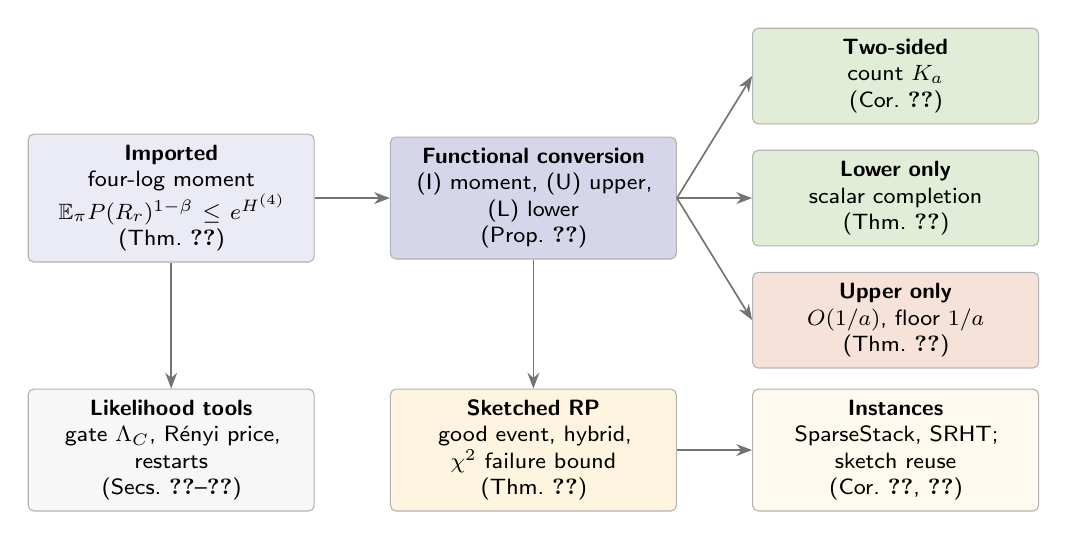
\begin{tikzpicture}[>=Stealth,font=\sffamily\footnotesize,
 box/.style={draw=black!30,rounded corners=2pt,fill=#1,align=center,
  text width=3.35cm,inner sep=4pt,minimum height=1.2cm},
 box/.default=black!2,
 arr/.style={->,draw=black!55,line width=.6pt}]
\node[box=NavyBlue!8] (imp) at (0,0) {\textbf{Imported}\\ four-log moment\\ $\E_\pi P(R_r)^{1-\beta}\le e^{H^{(4)}}$\\(Thm.~\ref{imp:four})};
\node[box=NavyBlue!16] (fun) at (4.6,0) {\textbf{Functional conversion}\\ (I) moment, (U) upper,\\ (L) lower\\ (Prop.~\ref{prop:functional})};
\node[box=OliveGreen!12] (two) at (9.2,1.55) {\textbf{Two-sided}\\ count $K_a$\\ (Cor.~\ref{cor:two-sided})};
\node[box=OliveGreen!12] (low) at (9.2,0) {\textbf{Lower only}\\ scalar completion\\ (Thm.~\ref{thm:lower})};
\node[box=BrickRed!10] (up) at (9.2,-1.55) {\textbf{Upper only}\\ $O(1/a)$, floor $1/a$\\ (Thm.~\ref{thm:upper})};
\node[box=Orange!12] (sk) at (4.6,-3.2) {\textbf{Sketched RP}\\ good event, hybrid,\\ $\chi^2$ failure bound\\ (Thm.~\ref{thm:sketch})};
\node[box=Orange!6] (inst) at (9.2,-3.2) {\textbf{Instances}\\ SparseStack, SRHT;\\ sketch reuse\\ (Cor.~\ref{cor:instances},~\ref{cor:reuse})};
\node[box=black!3] (gate) at (0,-3.2) {\textbf{Likelihood tools}\\ gate $\Lambda_C$, R\'enyi price,\\ restarts\\ (Secs.~\ref{sec:gate}--\ref{sec:restart})};
\draw[arr] (imp)--(fun);
\draw[arr] (fun.east)--(two.west);
\draw[arr] (fun.east)--(low.west);
\draw[arr] (fun.east)--(up.west);
\draw[arr] (fun)--(sk);
\draw[arr] (imp.south)--(gate.north);
\draw[arr] (sk)--(inst);
\end{tikzpicture}
\caption{Roadmap. The imported initial moment and the functional
conversion feed every pivot-count statement. The sketched theorem enters
the conversion through the same three inequalities as the two-sided
bracket, with $a=\gamma_\eta$.}
\label{fig:roadmap}
\end{figure}

\subsection{Organization}
Section~\ref{sec:prelim} collects the deterministic lemmas and the
imported moment theorem. Section~\ref{sec:robust} proves the functional
conversion phase by phase and the two-sided count.
Section~\ref{sec:trichotomy} proves the lower-only and upper-only
statements, including the floor construction. Section~\ref{sec:sketch}
treats sketched RPCholesky. Section~\ref{sec:gate} gives the
fixed-dictionary gate and Section~\ref{sec:restart} the restart
reduction. Section~\ref{sec:numerics} contains the numerical
illustrations and Section~\ref{sec:open} the open problems.

\subsection{Prior work and the contribution of this paper}
Chen, Epperly, Tropp and Webber~\cite{CETW} established the modern
RPCholesky analysis, including the exact conditional trace decrease.
The adaptive-sampling and volume-sampling arguments originate with
Deshpande and collaborators~\cite{DRVW,DV}. Our scalar phase and
pivot-product identities build on those arguments. The initial
fractional determinant moment is imported from~\cite{RA01}; this paper
does not claim a new proof of the exact-pivoting four-log bound.
The two-sided count itself is already Proposition 8.1 of that companion
paper. We reproduce it to expose the functional hypotheses needed below.

Divan and Gilles~\cite[Theorem 3.1]{DG} already analyze upper-dominated
laws $q\le\pi/\gamma$ through elementary symmetric polynomials. Their
sketchy RPLU analysis uses a fresh block at each iteration. The
contribution here is the functional reformulation of the companion
conversion, the complete one-sided trichotomy, and the finite-budget
floor under upper domination alone. For sketching,
we analyze RPCholesky on the Gram matrix of one reused sketch and measure
its selected-column error on the original matrix. Weighted tests replace
a coordinate union bound, and the hybrid chain transfers the drift
inequalities while charging failures through a likelihood second moment.

Epperly's analysis of adaptive randomized pivoting~\cite{EpperlyARP}
already identifies full-rank pivoting on an orthonormal frame with volume
sampling. Accordingly, the case $\Lambda_C=1$ of our frame gate is a
known identity, and its $k!$ bound is the comparison of~\cite{DV}. Our
refinement retains the residual spectral tails in $\Lambda_C$ and applies
the resulting price to sketch-assisted selection from a fixed dictionary.
Union amplification is an elementary independent-restart reduction;
its $O(r/\eps)$ consequence remains conditional on a uniform warm-start
moment. These distinctions are the basis of our novelty claims relative
to the works cited here.

\paragraph{Scope of the guarantees.}
The main trace bound concerns $A/J$, equivalently the best projection
onto the selected original columns. Reconstructing with the same sketch
has a separate good-event guarantee; it need not have controlled error
on failed histories. The explicit embedding constants are imported from
repository manuscripts~\cite{SparseStack,SRHThybrid}. Their use here is
conditional on those stated certificates, with each required estimate
restated in Section~\ref{sec:sketch}.
\section{Preliminaries and the imported moment}\label{sec:prelim}
All logarithms are natural. For a PSD matrix $R$ we write $\tau_j(R)$
for the sum of its eigenvalues beyond the $j$th. For an index set $J$
we write $A/J=A-A_{:J}A_{JJ}^{+}A_{J:}$ for the Schur complement
(residual) of $A$ after pivoting on $J$. Positive pivots never repeat an
index, and $A_{JJ}$ is then invertible, so $A/J$ does not depend on the
order of the pivots. Positive versions of the iterated logarithms are
\begin{equation}\label{eq:Lambda}
 \Lambda_1(r)=\log(e+r),\qquad
 \Lambda_{j+1}(r)=\log(e+\Lambda_j(r)).
\end{equation}
Fix $r\ge1$ with $\tau=\tau_r(A)>0$ and put
\[
 t=\frac r\tau,\qquad
 P(R)=\det(I+tR),\qquad
 p_R(z)=\det(I+zR).
\]
Since $\det(I+tR)\ge1+t\tr R$, we have $\tr R\le P(R)/t$.
The determinant potential controls exceptionally large residuals during
the warm-start phases. Once the expected trace is a constant multiple of
$\tau$, the trace decrease alone supplies the accuracy phase.
Every process is held at its terminal set after exhaustion; references
to $k$ steps mean at most $k$ positive pivots.

\subsection{Deterministic facts}
\begin{lemma}[Order and exhaustion]\label{lem:order}
Every positive pivot satisfies $0\preceq R^{(i)}\preceq R$ and lowers
the rank by one. Consequently every sequence of positive pivots
satisfies $\tr R_k\ge\tau_k(A)$ and $\tau_r(R_k)\le\tau_r(A)$, and
exhausts $A$ after $\rank A\le N$ pivots.
\end{lemma}
\begin{proof}
Put $u=R^{1/2}e_i/\sqrt{R_{ii}}$, a unit vector in the range of
$R^{1/2}$. Then $R^{(i)}=R^{1/2}(I-uu^*)R^{1/2}$, which is PSD, is
dominated by $R$, and has rank $\rank R-1$. The matrix $A-R_k$ is PSD,
dominated by $A$, and has rank at most $k$; hence its trace is at most
$\lambda_1+\dots+\lambda_k$, which is the first inequality. The second
follows from $R_k\preceq A$ and eigenvalue monotonicity.
\end{proof}

\begin{lemma}[Pivot products and exact path probabilities]\label{lem:path}
Let $w=(i_0,\dots,i_{k-1})$ be a sequence of positive pivots and
$J_s=\{i_0,\dots,i_{s-1}\}$. Then
\[
 \prod_{s<k}(A/J_s)_{i_si_s}=\det A_{J_kJ_k},\qquad
 \pi(w)=\frac{\det A_{J_kJ_k}}{\prod_{s<k}\tr(A/J_s)},
\]
where $\pi(w)$ is the probability that exact RPCholesky follows $w$.
\end{lemma}
\begin{proof}
The Schur determinant formula gives
$\det A_{J_{s+1}J_{s+1}}=\det A_{J_sJ_s}\,(A/J_s)_{i_si_s}$. Induction
gives the first identity, and the second is the product of the
transition probabilities~\eqref{eq:pi}.
\end{proof}

\begin{lemma}[Exact drifts]\label{lem:drifts}
Let $r\ge1$ and let $R\ne0$ be a residual with $T=\tr R$ and
$\tau_r(R)\le\tau$. Then
\begin{equation}\label{eq:exactdrifts}
 \begin{aligned}
 \E_\pi[P(R')\mid R]&=\frac{p_R'(t)}T,\\
 \E_\pi[\tr R'\mid R]&=T-\frac{\tr R^2}T.
 \end{aligned}
\end{equation}
and
\begin{equation}\label{eq:driftbounds}
 \begin{aligned}
 \frac{p_R'(t)}{T}&\le 2e\,P(R)^{1-1/r},\\
 \frac{p_R'(t)}{P(R)}&\le2\tau,\\
 \tr R^2&\ge\frac{(T-\tau)_+^2}r .
 \end{aligned}
\end{equation}
\end{lemma}
\begin{proof}
By the matrix determinant lemma,
$P(R^{(i)})=P(R)\bigl(1-t\,e_i^*R(I+tR)^{-1}Re_i/R_{ii}\bigr)$. Averaging
with weights $R_{ii}/T$ gives
$P(R)\bigl(1-(t/T)\tr[R^2(I+tR)^{-1}]\bigr)=(P(R)/T)\tr[R(I+tR)^{-1}]$,
and $\tr[R(I+tR)^{-1}]=p_R'(t)/P(R)$. The trace identity follows from
$\tr R^{(i)}=T-\|Re_i\|^2/R_{ii}$.

Let $x\tau$ be the sum of the $r$ largest eigenvalues of $R$ (padding
by zeros) and $y\tau$ the rest, so $0\le y\le1$ and $T=(x+y)\tau$.
AM--GM on the head and $\log(1+u)\le u$ on the tail give
$P(R)\le(1+x)^re^{ry}$. Concavity of $u\mapsto u/(1+tu)$ on the head
and $u/(1+tu)\le u$ on the tail give
$p_R'(t)/P(R)=\sum_j\lambda_j/(1+t\lambda_j)\le\tau[x/(1+x)+y]$. Hence
\[
 \frac{p_R'(t)}{T\,P(R)^{1-1/r}}
 \le\frac{\tau[x/(1+x)+y](1+x)e^y}{(x+y)\tau}
 =e^y\Bigl(1+\frac{xy}{x+y}\Bigr)\le e(1+y)\le2e .
\]
The bound $\lambda/(1+t\lambda)\le1/t$ on the $r$ head eigenvalues and
$\lambda/(1+t\lambda)\le\lambda$ on the tail give $p_R'(t)/P(R)\le
r/t+\tau=2\tau$. Finally the head eigenvalues sum to at least $T-\tau$,
so Cauchy--Schwarz gives $\tr R^2\ge(T-\tau)_+^2/r$.
\end{proof}

The trace excess is followed through the progress variable
\begin{equation}\label{eq:F}
 F(u)=\frac1u-\log u,\qquad u>0,
\end{equation}
which is decreasing and convex, with $F'(u)=-(1+u)/u^2$.

\begin{lemma}[Scalar completion]\label{lem:scalar}
Let $0<a\le1$, $r\ge1$, and $\phi_a(T)=T-a(T-\tau)_+^2/(rT)$ for
$T>0$, $\phi_a(0)=0$. Then $\phi_a$ is nondecreasing and concave on
$[0,\infty)$. If nonnegative numbers $f_k$ satisfy
$f_{k+1}\le\phi_a(f_k)$, then as long as $u_k=f_k/\tau-1>0$,
\[
 F(u_{k+1})\ge F(u_k)+\frac ar ,
\]
where $F(u_{k+1})=+\infty$ if $u_{k+1}\le0$. Consequently, if
$f_{k_0}\le(1+u)\tau$ with $u>\eps$, then $f_k\le(1+\eps)\tau$ for
$k\ge k_0+\lceil(r/a)(F(\eps)-F(u))\rceil$.
\end{lemma}
\begin{proof}
On $[0,\tau]$, $\phi_a(T)=T$. For $T>\tau$,
$\phi_a'(T)=1-(a/r)(1-\tau^2/T^2)\ge1-a/r\ge0$ and
$\phi_a''(T)=-2a\tau^2/(rT^3)<0$; the one-sided derivatives agree at
$\tau$. This proves monotonicity and concavity. Normalizing,
$u_{k+1}\le u_k-au_k^2/[r(1+u_k)]$, and the right side is positive.
Since $F$ is decreasing and convex,
\[
 F(u_{k+1})\ge F\Bigl(u_k-\frac{au_k^2}{r(1+u_k)}\Bigr)
 \ge F(u_k)-F'(u_k)\frac{au_k^2}{r(1+u_k)}=F(u_k)+\frac ar .
\]
Since $\phi_a(T)\le T$, the sequence $f_k$ is nonincreasing once it is
below $(1+\eps)\tau$, and the count follows.
\end{proof}

\subsection{The imported initial moment}
We use the following result as a black box. Put
$b_r=\log(1+2\log(r!)/r)$ and $a_r=r^r/r!$. For $r\ge2$ and
$0<\beta<1$, define the optimizing exponent and its logarithmic cost by
\begin{align*}
 \alpha_{r,\beta}&=\min\Bigl\{\beta,\frac{r-1}{rb_r}\Bigr\},\\
 B_{r,\beta}&=rb_r\alpha_{r,\beta}-(r-1)\log\alpha_{r,\beta}.
\end{align*}
Let $\varphi=(1+\sqrt5)/2$ and
$\cvol=1+2\log\varphi+\varphi^{-1}$. The imported moment scale is
\begin{equation}\label{eq:H4}
 H_{r,\beta}^{(4)}=B_{r,\beta}+\log a_r+\beta r\log2+(1-\beta)\cvol r .
\end{equation}

\begin{imported}[{\cite[Proposition 7.2 and Theorem 6.3]{RA01}}]\label{imp:four}
Let $r\ge2$ and $0<\beta<1$. For every finite PSD matrix $A$ with
$\tau_r(A)>0$, exact RPCholesky satisfies
\begin{equation}\label{eq:imp-moment}
 \E_\pi P(R_r)^{1-\beta}\le\exp\bigl(H_{r,\beta}^{(4)}\bigr).
\end{equation}
Moreover, for every PSD $A$ with $\rank A\ge r$ (including
$\rank A=r$), let $\mu_r$ be the law of the unordered set of the first
$r$ pivots, $\nu_r(S)=\det A_{SS}/e_r(A)$ the volume-sampling law, and
$L_A=\mu_r/\nu_r$. Then
\begin{equation}\label{eq:imp-renyi}
 \E_{\nu_r}L_A^{1/\beta}\le e^{B_{r,\beta}/\beta}\,2^r\,a_r^{1/\beta}.
\end{equation}
For fixed $\beta$, $B_{r,\beta}=O(r\log\log\log r)$ and
$H_{r,\beta}^{(4)}/r=O(\log\log\log r)$.
\end{imported}

The same paper converts~\eqref{eq:imp-moment} into the count
$K_4(r,\eps)=O(r/\eps+r\Lambda_4(r))$ for exact RPCholesky; its
conversion is the case $a=1$ of Proposition~\ref{prop:functional} below,
and the resulting counts at $\eps=1$ are $71$, $722$, $7243$, $72539$
and $726105$ for $r=10,10^2,\dots,10^5$, with $\beta$ optimized for
each rank. We have recomputed these values.
\section{A functional robust conversion}\label{sec:robust}
Throughout this section $(R_k)_{k\ge0}$ is a sequence of residuals of
$A$ produced by positive pivots and exact Schur updates, adapted to a
filtration $(\calF_k)$. The filtration contains the pivots chosen so far
and may contain arbitrary external randomness, such as a sketching
matrix. No independence between steps is assumed.

\subsection{Statement}
Fix $r\ge2$, $\tau=\tau_r(A)>0$, $0<\eps\le1$, $0<a\le1$, $0<\theta\le1$
and a real number $H$. Put $\zeta=1-1/r$.
The four phase lengths are $r$, $g_a$, $s_a$ and $n_a$. We define them
in their order of use. Cooling reduces the moment exponent:
\begin{equation}\label{eq:g}
 c_a=\log(2e/a),\qquad
 g_a=\left\lceil\frac{\log\max\bigl\{\theta^{-1},\,[H/(r\theta)-c_a]/\log5,\,1\bigr\}}
                   {-\log(1-1/r)}\right\rceil.
\end{equation}
Its remaining first-moment scale is
\begin{equation}\label{eq:D}
 \rho_a=\zeta^{g_a},\qquad
 D_a=(1-\rho_a)rc_a+\rho_aH/\theta.
\end{equation}
The stopping phase reaches a constant expected trace excess:
\begin{equation}\label{eq:s}
 s_a=\lceil D_a/\log5\rceil,\qquad u_a=10/a-1+1/r.
\end{equation}
Finally, the scalar progress function fixes the accuracy phase:
\begin{equation}\label{eq:calK}
 \begin{aligned}
 n_a&=\left\lceil\frac ra\bigl(F(\eps)-F(u_a)\bigr)\right\rceil,\\
 \calK_a(r,\eps;\theta,H)&=r+g_a+s_a+n_a.
 \end{aligned}
\end{equation}
At $a=1$ these are exactly the formulas of the exact-probability
conversion in~\cite{RA01}.

\begin{proposition}[Functional robust conversion]\label{prop:functional}
Assume
\begin{enumerate}[label=\textup{(\Roman*)},leftmargin=2.2em]
\item[\textup{(I)}] $\E P(R_r)^\theta\le e^H$;
\item[\textup{(U)}] for every $k\ge r$, on $\{R_k\ne0\}$,
 $\E[P(R_{k+1})\mid\calF_k]\le a^{-1}p_{R_k}'(t)/\tr R_k$;
\item[\textup{(L)}] for every $k\ge r$, on $\{R_k\ne0\}$,
 $\E[\tr R_{k+1}\mid\calF_k]\le\tr R_k-a\tr R_k^2/\tr R_k$.
\end{enumerate}
Then $\E\tr R_k\le(1+\eps)\tau$ for every
$k\ge\min\{N,\calK_a(r,\eps;\theta,H)\}$.
\end{proposition}

By~\eqref{eq:exactdrifts}, the right sides of (U) and (L) are $a^{-1}$
times the exact conditional mean of $P(R')$, and the exact mean trace
decrease multiplied by $a$. The hypotheses therefore compare only two
functionals of the pivot law with their exact values: the determinant
functional $i\mapsto P(R^{(i)})$ from above, and the trace decrease
$i\mapsto\|Re_i\|^2/R_{ii}$ from below.

\subsection{Proof, phase by phase}
The residual is zero from some time on only if it is exhausted, and a
zero residual stays zero; on $\{R_k=0\}$ all the bounds below hold
trivially because $P(0)=1$ and $\tr 0=0$. After $\rank A\le N$
positive pivots the residual is zero, which gives the cap at $N$.
Pathwise $\tr R_k$ is nonincreasing (Lemma~\ref{lem:order}), so it
suffices to prove the bound at $k=\calK_a$.

\paragraph{Phase 1: initialization ($r$ pivots).}
This phase is hypothesis (I).

\paragraph{Phase 2: cooling ($g_a$ pivots).}
By (U) and the first inequality in~\eqref{eq:driftbounds}, for $k\ge r$,
\[
 \E[P(R_{k+1})\mid\calF_k]\le\frac{2e}a\,P(R_k)^{\zeta}.
\]
We claim that for $j\ge0$,
$\E[P(R_{r+j})\mid\calF_r]\le(2e/a)^{r(1-\zeta^j)}P(R_r)^{\zeta^j}$.
For $j=0$ this is trivial. If it holds for $j$, then by the tower
property and conditional Jensen for the concave map $x\mapsto x^\zeta$,
\[
 \E[P(R_{r+j+1})\mid\calF_r]
 \le\frac{2e}a\E[P(R_{r+j})^\zeta\mid\calF_r]
 \le\frac{2e}a\Bigl((2e/a)^{r(1-\zeta^j)}P(R_r)^{\zeta^j}\Bigr)^\zeta,
\]
and $1+r\zeta(1-\zeta^j)=r(1-\zeta^{j+1})$ because $r(1-\zeta)=1$.
Take $j=g_a$. The first entry of the maximum in~\eqref{eq:g} gives
$\rho_a\le\theta$, so Jensen and (I) give
\[
 \log\E P(R_{r+g_a})\le(1-\rho_a)rc_a+\log\E P(R_r)^{\rho_a}
 \le(1-\rho_a)rc_a+\frac{\rho_a}\theta\log\E P(R_r)^{\theta}\le D_a .
\]
The second entry gives $\rho_a[H/(r\theta)-c_a]\le\log5$, which is
$D_a\le r(c_a+\log5)$.

\paragraph{Phase 3: stopping ($s_a$ pivots).}
Let $k\ge r+g_a$ and suppose $\tr R_k>10\tau/a$. By (U) and the second
inequality in~\eqref{eq:driftbounds},
\[
 \E[P(R_{k+1})\mid\calF_k]\le\frac{2\tau}{a\tr R_k}P(R_k)\le\frac15P(R_k).
\]
Put $Z_k=P(R_k)\1\{\tr R_k>10\tau/a\}$. Since the trace is pathwise
nonincreasing, $\1\{\tr R_{k+1}>10\tau/a\}\le\1\{\tr R_k>10\tau/a\}$,
and therefore $\E[Z_{k+1}\mid\calF_k]\le Z_k/5$. After $s_a$ steps
$\E Z_{r+g_a+s_a}\le5^{-s_a}e^{D_a}\le1$. Since $\tr R\le P(R)/t$,
\[
 \E\tr R_{r+g_a+s_a}\le\frac{10\tau}a+\frac{\E Z_{r+g_a+s_a}}t
 \le\Bigl(\frac{10}a+\frac1r\Bigr)\tau=(1+u_a)\tau .
\]

\paragraph{Phase 4: accuracy ($n_a$ pivots).}
By (L), Lemma~\ref{lem:order} ($\tau_r(R_k)\le\tau$) and the last
inequality in~\eqref{eq:driftbounds},
$\E[\tr R_{k+1}\mid\calF_k]\le\phi_a(\tr R_k)$ with $\phi_a$ as in
Lemma~\ref{lem:scalar}. Since $\phi_a$ is concave and nondecreasing,
Jensen gives $f_{k+1}\le\phi_a(f_k)$ for the means $f_k=\E\tr R_k$.
Lemma~\ref{lem:scalar}, started from $u\le u_a$, gives
$f_k\le(1+\eps)\tau$ after $n_a$ further pivots. This proves the
proposition. \qed

\begin{remark}[Which side is used where]\label{rem:sides}
Phases~2 and~3 use only (U), an upper comparison. Phase~4 uses only (L),
a lower comparison. Phase~1 is a moment hypothesis; under a
per-coordinate bracket it is obtained from the upper side through the
path likelihood. This separation is the source of the trichotomy in
Section~\ref{sec:trichotomy}.
\end{remark}

\subsection{Two-sided brackets}
\begin{corollary}[Two-sided robust count, recalled from {\cite[Proposition 8.1]{RA01}}]\label{cor:two-sided}
Let $r\ge2$ and suppose that, conditionally on the complete past, the
pivot law satisfies
\begin{equation}\label{eq:two-sided}
 a\pi_i\le q_i\le a^{-1}\pi_i\qquad\text{for all }i,\qquad 0<a\le1.
\end{equation}
If exact RPCholesky satisfies $\E_\pi P(R_r)^\theta\le e^H$, then
$\E\tr R_k\le(1+\eps)\tau$ for all
$k\ge\min\{N,K_a\}$, where
\[
 K_a=r+g_a+s_a+n_a=\calK_a\bigl(r,\eps;\theta,H+r\log(1/a)\bigr).
\]
With Imported Theorem~\ref{imp:four}, $\theta=1-\beta$ and
$H=H^{(4)}_{r,\beta}$, for fixed $0<\beta<1$,
\begin{equation}\label{eq:Ka-asympt}
 K_a=O\Bigl(\frac r{a\eps}+\frac ra\log\frac ea+r\Lambda_4(r)\Bigr),
\end{equation}
with a constant independent of $a$, $\eps$ and $r$.
\end{corollary}
\begin{proof}
\emph{(I).} By induction on the steps, the probability that the process
follows a pivot sequence $w$ of length $r$ is at most $a^{-r}\pi(w)$:
each conditional factor $q(i_s\mid\calF_s)$ is at most
$a^{-1}\pi(i_s\mid J_s)$, and $\pi(\cdot\mid J_s)$ depends only on the
set $J_s$. Since $P(R_r)^\theta\ge0$ is a function of the sequence,
$\E_qP(R_r)^\theta\le a^{-r}\E_\pi P(R_r)^\theta\le e^{H+r\log(1/a)}$.

\emph{(U).} $P(R^{(i)})\ge0$, so
$\sum_iq_iP(R^{(i)})\le a^{-1}\sum_i\pi_iP(R^{(i)})=a^{-1}p_R'(t)/\tr R$
by~\eqref{eq:exactdrifts}.

\emph{(L).} The decrease $\|Re_i\|^2/R_{ii}$ is nonnegative, so
$\sum_iq_i\|Re_i\|^2/R_{ii}\ge a\sum_i\pi_i\|Re_i\|^2/R_{ii}
=a\tr R^2/\tr R$.

Proposition~\ref{prop:functional} gives the count. For the asymptotics,
$u_a\le10/a$ and $F(u_a)\ge-\log u_a$, so
$n_a\le1+(r/a)(\eps^{-1}+\log\eps^{-1}+\log(10/a))$. Next
$D_a\le r(c_a+\log5)$ gives $s_a=O(r\log(e/a))$. Finally
$-1/\log(1-1/r)\le r$ and $H^{(4)}_{r,\beta}/r=O(\log\log\log r)$ give
\[
 g_a\le1+r\log\max\Bigl\{\frac1{1-\beta},\,
 C\bigl(1+\log\log\log(e^e+r)+\log(1/a)\bigr)\Bigr\}
 =O\bigl(r\Lambda_4(r)+r\log(e/a)\bigr),
\]
using $\log(x+y)\le\log x+\log(1+y)$ for $x\ge1$, $y\ge0$. Since
$\log\eps^{-1}\le\eps^{-1}$ and $r\log(e/a)\le(r/a)\log(e/a)$, the
bound~\eqref{eq:Ka-asympt} follows.
\end{proof}

\begin{remark}[Rank one and zero tails]\label{rem:rank-one}
For $r=1$ the upper side applied to the nonnegative function
$i\mapsto\tr R^{(i)}$ at the first step gives
$\E_q\tr R_1\le a^{-1}\E_\pi\tr R_1\le2\tau_1(A)/a$, because
$\E_\pi\tr R_1\le(\lambda_1+\tau)-\lambda_1^2/(\lambda_1+\tau)\le2\tau$.
Lemma~\ref{lem:scalar} with $r=1$ then shows that
$1+\lceil a^{-1}[F(\eps)-F(2/a-1)]\rceil$ pivots suffice. If
$\tau_r(A)=0$, positive pivots exhaust $A$ after at most $r$ steps.
Any count valid for rank $2$ is also valid for the rank-one target,
since $\tau_2(A)\le\tau_1(A)$.
\end{remark}

At $a=1$ the corollary is the four-logarithm theorem of~\cite{RA01}.
Table~\ref{tab:Ka} in Section~\ref{sec:numerics} evaluates $K_a$: at
$r=1000$ and $\eps=1$ the count grows from $7243$ at $a=1$ to $12393$ at
$a=1/2$, and at $\eps=0.1$ from $18545$ to $34998$. The dominant change
is the factor $1/a$ in the accuracy phase.
\section{The robustness trichotomy}\label{sec:trichotomy}
Remark~\ref{rem:sides} says which side of the bracket each phase uses.
This section shows that the division is sharp: a lower bracket alone
keeps the final accuracy phase, and an upper bracket alone keeps the
first three phases but not the accuracy.

\begin{figure}[t]
\centering
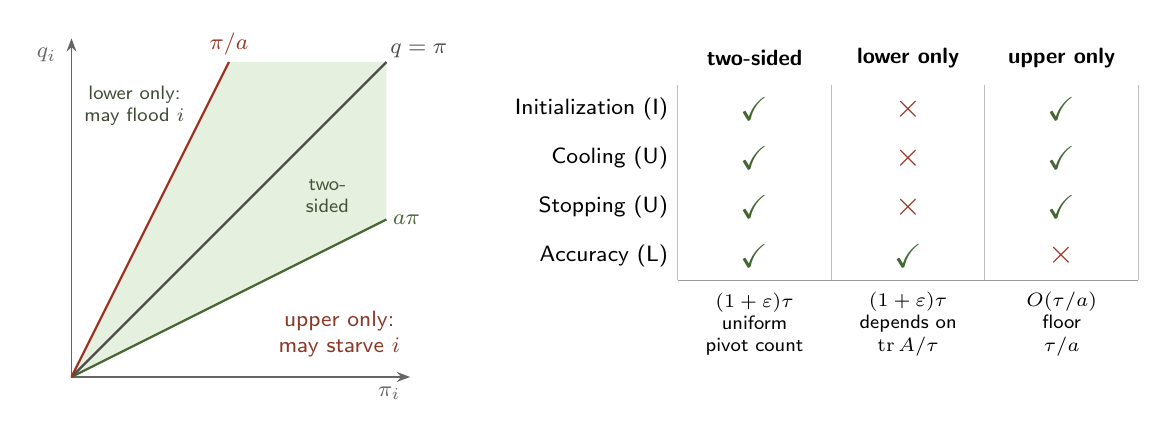
\begin{tikzpicture}[>=Stealth,font=\sffamily\footnotesize]
\begin{scope}
\draw[->,black!60] (0,0)--(4.3,0) node[below left]{$\pi_i$};
\draw[->,black!60] (0,0)--(0,4.3) node[below left,xshift=-2pt]{$q_i$};
\fill[OliveGreen!10] (0,0)--(4,2)--(4,4)--(2,4)--cycle;
\draw[black!70,thick] (0,0)--(4,4) node[above right,inner sep=1pt]{$q=\pi$};
\draw[OliveGreen!70!black,thick] (0,0)--(4,2) node[right,inner sep=2pt]{$a\pi$};
\draw[BrickRed!80!black,thick] (0,0)--(2,4) node[above,inner sep=2pt]{$\pi/a$};
\node[align=center,text=OliveGreen!50!black,font=\sffamily\scriptsize] at (3.25,2.3) {two-\\sided};
\node[align=center,text=BrickRed!70!black] at (3.4,0.55) {upper only:\\ may starve $i$};
\node[align=center,text=OliveGreen!40!black,font=\sffamily\scriptsize] at (0.8,3.45) {lower only:\\ may flood $i$};
\end{scope}
\begin{scope}[xshift=7.7cm,yshift=.1cm]
\def\cw{1.95}\def\rh{.62}
\foreach \j/\t in {0/{Initialization (I)},1/{Cooling (U)},2/{Stopping (U)},3/{Accuracy (L)}}
 \node[anchor=east] at (0,{3.3-\j*\rh}) {\t};
\foreach \i/\t in {1/{two-sided},2/{lower only},3/{upper only}}
 \node[font=\sffamily\footnotesize\bfseries] at ({(\i-.5)*\cw},3.95) {\t};
\foreach \i in {0,1,2,3} \draw[black!25] ({\i*\cw},{3.3+\rh/2})--({\i*\cw},{3.3-3.5*\rh});
\newcommand{\yes}[2]{\node[text=OliveGreen!70!black] at ({(#1-.5)*\cw},{3.3-#2*\rh}) {\large$\checkmark$};}
\newcommand{\no}[2]{\node[text=BrickRed!80!black] at ({(#1-.5)*\cw},{3.3-#2*\rh}) {\large$\times$};}
\yes10\yes11\yes12\yes13
\no20\no21\no22\yes23
\yes30\yes31\yes32\no33
\draw[black!40] (0,{3.3-3.5*\rh})--({3*\cw},{3.3-3.5*\rh});
\node[align=center,font=\sffamily\scriptsize] at ({.5*\cw},{3.3-4.4*\rh}) {$(1+\eps)\tau$\\ uniform\\ pivot count};
\node[align=center,font=\sffamily\scriptsize] at ({1.5*\cw},{3.3-4.4*\rh}) {$(1+\eps)\tau$\\ depends on\\ $\tr A/\tau$};
\node[align=center,font=\sffamily\scriptsize] at ({2.5*\cw},{3.3-4.4*\rh}) {$O(\tau/a)$\\ floor\\ $\tau/a$};
\end{scope}
\end{tikzpicture}
\caption{The robustness trichotomy. Left: the admissible region for a
pivot probability $q_i$ given $\pi_i$. Right: which phases of the
conversion survive, and the resulting guarantee. The lower-only count
contains $\log(\tr A/\tau)$ and starts from the input (or from any warm
start); the upper-only floor is Theorem~\ref{thm:upper}(b).}
\label{fig:trichotomy}
\end{figure}

\subsection{Lower brackets}
\begin{theorem}[Lower brackets keep the scalar completion]\label{thm:lower}
Let $r\ge1$, $\tau=\tau_r(A)>0$, $0<a\le1$, and suppose the pivot law
satisfies $q_i\ge a\pi_i$ for all $i$, conditionally on the complete
past. If $\E\tr R_{k_0}\le(1+u)\tau$ with $u>\eps$, then
$\E\tr R_k\le(1+\eps)\tau$ for all
$k\ge k_0+\lceil(r/a)(F(\eps)-F(u))\rceil$. In particular
\[
 k\ge\Bigl\lceil\frac ra\Bigl(\frac1\eps+\log\frac1\eps
 +\log\frac{\tr A}\tau\Bigr)\Bigr\rceil
\]
pivots suffice from $R_0=A$.
\end{theorem}
\begin{proof}
The proof of (L) in Corollary~\ref{cor:two-sided} uses only the lower
side, so (L) holds at every step. Phase~4 of the proof of
Proposition~\ref{prop:functional} applies verbatim from time $k_0$.
From $R_0=A$ we have $u=\tr A/\tau-1$ and
$F(u)>-\log u>-\log(\tr A/\tau)$, while
$F(\eps)=\eps^{-1}+\log\eps^{-1}$.
\end{proof}

Thus a lower bracket never produces an accuracy floor: every relative
accuracy is reached, at a count that depends on the starting excess only
logarithmically. What is lost is the uniformity in $\tr A/\tau$: the
determinant phases that remove this dependence need an upper comparison.

\subsection{Upper brackets}
\begin{theorem}[Upper brackets: constant factor, and a floor]\label{thm:upper}
Let $0<a\le1$.
\begin{enumerate}[label=\textup{(\alph*)}]
\item Let $r\ge2$ and $\tau=\tau_r(A)>0$. If $q_i\le\pi_i/a$ for all $i$,
 conditionally on the complete past, and exact RPCholesky satisfies
 $\E_\pi P(R_r)^\theta\le e^H$, then $\E\tr R_k\le(10/a+1/r)\tau$ for all
 $k\ge r+g_a+s_a$, with $g_a,s_a$ computed from $(\theta,H+r\log(1/a))$.
\item For every $r\ge1$, every budget $k\ge0$ and every $\delta>0$ there
 are $m$ and a memoryless pivot rule with $q\le\pi/a$ such that, on
 \[
  A=\diag(\Theta I_r,I_m),\qquad \Theta=\frac{(m-k)(1-a)}{ar},
 \]
 the residual after $k$ pivots is deterministic and
 \[
  \frac{\tr R_k}{\tau_r(A)}\ge\frac{1-k/m}a\ge\frac1a-\delta .
 \]
\end{enumerate}
\end{theorem}
\begin{proof}
(a) The proof of (I) and (U) in Corollary~\ref{cor:two-sided} uses only
the upper side. Phases~1--3 of Proposition~\ref{prop:functional} then
give the stated bound, and the trace is nonincreasing afterwards.

(b) Take $m>k+r$ and $m\ge k/(a\delta)$. This ensures a positive
rank-$r$ tail even when $a=1$, for which $\Theta=0$. Label the first $r$ coordinates
\emph{heads} and the last $m$ \emph{tails}. Every residual reached by
positive pivots on a diagonal matrix is the same diagonal matrix with
the pivoted coordinates removed; a state is described by the numbers $h$
of heads and $b$ of tails that remain. The rule is as follows: if
$b\ge1$ and $h\Theta\le b(1-a)/a$, choose a remaining tail uniformly;
otherwise use exact RPCholesky. In the first case, a remaining tail $i$
has $q_i=1/b$ and $\pi_i=1/(h\Theta+b)$, and $q_i\le\pi_i/a$ is equivalent to
$a(h\Theta+b)\le b$, which is the case condition; heads have $q_i=0$. So the
rule satisfies $q\le\pi/a$ at every state.

Start from $h=r$, $b=m$. Before the $(s+1)$st pivot, $s<k$, we have
$b=m-s\ge m-k+1$ and $r\Theta=(m-k)(1-a)/a\le b(1-a)/a$, so the rule picks a
tail. After $k$ pivots the residual is $\diag(\Theta I_r,I_{m-k})$ and
\[
 \tr R_k=r\Theta+m-k=\frac{(m-k)(1-a)}a+(m-k)=\frac{m-k}a .
\]
The eigenvalues of $A$ are $\Theta$ ($r$ times) and $1$ ($m$ times), so
$\tau_r(A)\le m$ in either order. Hence
$\tr R_k/\tau_r(A)\ge(1-k/m)/a\ge1/a-\delta$.
\end{proof}

\begin{remark}\label{rem:floor}
In the construction the heads are starved: $q=0<a\pi$ on them. Any
lower bracket rules this out, and Theorem~\ref{thm:lower} then forces
the error to $(1+\eps)\tau$. Conversely, the construction does not
contradict part~(a): when $\Theta\ge1$, $\tau_r(A)=m$ and
$\tr R_k\le\tr A\le m/a$ for every $k$, so the floor $1/a$ is also the
largest possible ratio on this family.
The floor holds at every finite budget, but the input depends on the
budget through $m$. Section~\ref{sec:numerics} evaluates, by an exact
dynamic program, the four laws on this family: exact, two-sided,
lower-only and upper-only adversaries.
\end{remark}

\begin{proof}[Proof of Theorem~\ref{thm:intro-tri}]
Part~(i) is Corollary~\ref{cor:two-sided} for $r\ge2$ and
Remark~\ref{rem:rank-one} for $r=1$. Part~(ii) is
Theorem~\ref{thm:lower}. Part~(iii) is Theorem~\ref{thm:upper}.
\end{proof}
\section{Sketched RPCholesky}\label{sec:sketch}
\subsection{The algorithm and two exact identities}
Let $F\in\C^{D\times N}$ and $A=F^*F$. Let $\Pi\in\C^{m\times D}$ be a
random matrix, independent of the pivot randomness, and put
$B=F^*\Pi^*\Pi F$. \emph{Sketched RPCholesky} runs exact RPCholesky on
$B$: at a pivot set $J$ with $\tr(B/J)>0$ it chooses $i$ with probability
\[
 q_\Pi(i\mid J)=\frac{(B/J)_{ii}}{\tr(B/J)},
\]
and it stops early if $\tr(B/J)=0$. A stopped chain keeps its final set
at all later times; an exhausted reference or hybrid chain uses the
same convention. After $K$ steps it returns the set
$J$; the error is measured on $A$ by $\tr(A/J)$. It may also return the
same-sketch reconstruction
\[
 X_B=(\Pi F_J)^+\Pi F,\qquad F\approx F_JX_B .
\]
We write $R_A(J)=A/J$ and $R_B(J)=B/J$.

For a set $J$ such that $F_J$ has full column rank, let $Q_J\in\C^{D\times|J|}$
have orthonormal columns spanning the range of $F_J$, and put
\[
 E_J=(I-Q_JQ_J^*)F,\qquad G_J=Q_J^*\Pi^*\Pi Q_J .
\]
Then $R_A(J)=E_J^*E_J$. When $G_J$ is invertible, let
$P_J=\Pi Q_JG_J^{-1}Q_J^*\Pi^*$ be the orthogonal projector onto the
range of $\Pi Q_J$, which is the range of $\Pi F_J$.

\begin{lemma}[Sketched residual]\label{lem:sk-residual}
If $F_J$ and $\Pi F_J$ have full column rank, then
\[
 R_B(J)=(\Pi E_J)^*(I-P_J)(\Pi E_J).
\]
In particular $(R_B(J))_{ii}=\|(I-P_J)\Pi E_Je_i\|^2$, and
$(R_A(J))_{ii}=0$ implies $(R_B(J))_{ii}=0$. Along every path of
sketched RPCholesky, $F_J$ and $\Pi F_J$ keep full column rank, and
every pivot is positive for both $A$ and $B$.
\end{lemma}
\begin{proof}
The Schur complement of a Gram matrix is the Gram matrix of the
projected residual: $B/J=(\Pi F)^*(I-P_J)(\Pi F)$. Write
$F=F_JX+E_J$ with $X=(F_J^*F_J)^{-1}F_J^*F$; then
$\Pi F=\Pi F_JX+\Pi E_J$ and $(I-P_J)\Pi F_J=0$. If $(R_A)_{ii}=0$ then
$E_Je_i=0$. A pivot $i$ is chosen only if $(R_B)_{ii}>0$, which means
$\Pi Fe_i\notin\operatorname{range}\Pi F_J$; hence $\Pi F_{J\cup\{i\}}$,
and therefore $F_{J\cup\{i\}}$, has full column rank, and
$(R_A)_{ii}>0$. Induction on the steps completes the proof.
\end{proof}

\begin{lemma}[Exact path-likelihood identity]\label{lem:likelihood}
Let $w=(i_0,\dots,i_{t-1})$ be a pivot sequence with positive pivots
for $B$, and let $J_s=\{i_0,\dots,i_{s-1}\}$. Let $q_\Pi(w)$ and $p(w)$
be the probabilities that sketched RPCholesky and exact RPCholesky on
$A$ follow $w$. Then
\[
 \frac{q_\Pi(w)}{p(w)}
 =\det\bigl(Q_{J_t}^*\Pi^*\Pi Q_{J_t}\bigr)
  \prod_{s<t}\frac{\tr R_A(J_s)}{\tr R_B(J_s)} .
\]
\end{lemma}
\begin{proof}
Lemma~\ref{lem:path} for $A$ and for $B$ gives
$q_\Pi(w)=\det B_{J_tJ_t}/\prod_s\tr R_B(J_s)$ and
$p(w)=\det A_{J_tJ_t}/\prod_s\tr R_A(J_s)$. Write $F_{J_t}=Q_{J_t}C$
with $C$ invertible. Then $A_{J_tJ_t}=C^*C$ and
$B_{J_tJ_t}=C^*G_{J_t}C$, so the ratio of determinants is
$\det G_{J_t}$.
\end{proof}

The identity shows that sketched pivoting reads only two things: the
distortion of the path subspace $\operatorname{range}F_{J_t}$, and the
ratio of residual traces along the path. Both are properties of
subspaces of dimension at most $t+1$, and the reference law $p$ does not
depend on $\Pi$.

\subsection{The moment property}
For an isometry $U$ put $Z_U=U^*\Pi^*\Pi U-I$.

\begin{definition}\label{def:MP}
The random matrix $\Pi$ has the \emph{moment property}
$\MP(d,\ell,\eps_0)$ if
$\E\tr Z_U^{2\ell}\le d\,\eps_0^{2\ell}$ for every isometry
$U\in\C^{D\times d'}$ with $d'\le d$.
\end{definition}

\begin{remark}\label{rem:MP}
(i) If $D\ge d$ and the bound holds for every isometry with exactly $d$
columns, it holds for fewer columns: extend $U$ to an isometry $U'$ with
$d$ columns; then $Z_U$ is a compression of $Z_{U'}$, and Schatten norms
do not increase under compression, so
$\tr Z_U^{2\ell}\le\tr Z_{U'}^{2\ell}$. If $D<d$, pad $F$ with zero
rows; for sketches with independent columns, such as SparseStack, this
does not change $\Pi F$ in law.
(ii) A real sketch applied to complex data: if $U$ is a complex isometry
with $d$ columns, let $W$ be a real isometry whose range is the real
span of the real and imaginary parts of the columns of $U$; it has at
most $2d$ columns and $U=WC$ with $C^*C=I$. Then $Z_U=C^*Z_WC$, so
$\MP(2d,\ell,\eps_0)$ for real isometries gives the complex bound
$\E\tr Z_U^{2\ell}\le2d\,\eps_0^{2\ell}$. This has twice the prefactor
in Definition~\ref{def:MP}; it is not literally $\MP(d,\ell,\eps_0)$.
The bad-state bound is therefore doubled, and the first-failure bound
is multiplied by $\sqrt2$. Increasing the prescribed $\ell$ by one
absorbs that factor.
(iii) Markov's inequality and $\|Z\|^{2\ell}\le\tr Z^{2\ell}$ give
$\Prob\{\|Z_U\|>\eta\}\le d(\eps_0/\eta)^{2\ell}$, the usual subspace
embedding statement.
\end{remark}

\subsection{The good event on path-local subspaces}
Fix $K\ge1$, $0<\eta\le1/4$, a set $J$ with $|J|\le K$ such that $F_J$
has full column rank, and suppose $R_A(J)\ne0$. Let $\Sigma_J$ be the set
of $i$ with $(R_A(J))_{ii}>0$. For $i\in\Sigma_J$ put
\[
 u_i=\frac{E_Je_i}{\|E_Je_i\|},\qquad U_i=[\,Q_J\ \ u_i\,],\qquad
 Z_i=U_i^*\Pi^*\Pi U_i-I .
\]
Since $Q_J^*u_i=0$, $U_i$ is an isometry with at most $K+1$ columns.
Define three probability vectors on $\Sigma_J$:
\begin{align*}
 \omega^{(1)}_i&=\frac{(R_A)_{ii}}{\tr R_A},\\
 \omega^{(2)}_i&=\frac{\|R_Ae_i\|^2}{\tr R_A^2},\\
 \omega^{(3)}_i&=\frac{(R_A)_{ii}P(R_A^{(i)})}{\sum_j(R_A)_{jj}P(R_A^{(j)})}.
\end{align*}
where $R_A=R_A(J)$, $R_A^{(i)}=A/(J\cup\{i\})$, and $P$ is the
determinant potential of Section~\ref{sec:prelim}. The first is the exact
pivot law, the second weights the exact trace decrease, and the third
weights the exact determinant drift. For $c=1,2,3$ put
\[
 \Phi_c(J)=\sum_{i\in\Sigma_J}\omega^{(c)}_i\|Z_i\|^4 .
\]
The \emph{good event} at $J$ is
\begin{equation}\label{eq:good}
 \calG(J)=\bigl\{\|G_J-I\|\le\eta\bigr\}\cap
 \bigl\{\Phi_c(J)\le\eta^4/4\ \text{ for }c=1,2,3\bigr\}.
\end{equation}
If $R_A(J)=0$ we set $\calG(J)$ to be the sure event. The frames $U_i$
and the weights $\omega^{(c)}$ are determined by $F$, $J$, $r$ and
$\tau$; they do not depend on $\Pi$. A state is \emph{bad} if its good
event fails.

\begin{lemma}[Bad states are rare]\label{lem:bad}
Let $\Pi$ have $\MP(K+1,\ell,\eps_0)$ with $\ell\ge2$ and
$\eps_0\le\eta/2$. For every fixed $J$ with $|J|\le K$,
\[
 \Prob\{\calG(J)^c\}\le(K+1)\Bigl[\Bigl(\frac{\eps_0}\eta\Bigr)^{2\ell}
 +3\Bigl(\frac{2\eps_0^2}{\eta^2}\Bigr)^\ell\Bigr]
 \le4(K+1)2^{-\ell}=:\delta_1 .
\]
\end{lemma}
\begin{proof}
Remark~\ref{rem:MP}(iii) bounds the first event. For the others,
$\|Z_i\|^{2\ell}\le\tr Z_i^{2\ell}$ gives
$\E\|Z_i\|^{2\ell}\le(K+1)\eps_0^{2\ell}$. Since $\ell/2\ge1$,
Minkowski's inequality in $L^{\ell/2}$ applied to the nonnegative
variables $\omega_i^{(c)}\|Z_i\|^4$ gives
\[
 \bigl(\E\Phi_c^{\ell/2}\bigr)^{2/\ell}
 \le\sum_i\omega^{(c)}_i\bigl(\E\|Z_i\|^{2\ell}\bigr)^{2/\ell}
 \le\bigl((K+1)\eps_0^{2\ell}\bigr)^{2/\ell}.
\]
Markov's inequality gives
$\Prob\{\Phi_c>\eta^4/4\}\le(K+1)\eps_0^{2\ell}(4/\eta^4)^{\ell/2}
=(K+1)(2\eps_0^2/\eta^2)^\ell$. With $\eps_0\le\eta/2$ the four terms
are at most $(K+1)(4^{-\ell}+3\cdot2^{-\ell})\le4(K+1)2^{-\ell}$.
\end{proof}

No union bound over the $N$ coordinates occurs: each of the four events
is a statement about one weighted average over coordinates, and
Minkowski's inequality averages the per-coordinate moment bounds.
\subsection{What a good state guarantees}
Put
\begin{equation}\label{eq:gamma-chi}
 \gamma_\eta=\frac{1-\eta-\eta^2}{1+\eta},\qquad
 \chi_\eta^2=\frac{\bigl(\eta/\sqrt2+\eta^2/(2(1-\eta))\bigr)^2}{(1-\eta-\eta^2)^2}.
\end{equation}
For $\eta=0.1$ and $\eta=1/4$ these are $\gamma_\eta=0.809$,
$\chi^2_\eta=0.0073$ and $\gamma_\eta=0.55$, $\chi^2_\eta=0.101$. As
$\eta\to0$, $1-\gamma_\eta\sim2\eta$ and $\chi^2_\eta\sim\eta^2/2$.

\begin{lemma}[Consequences of a good state]\label{lem:good}
Let $\calG(J)$ hold, $R_A(J)\ne0$, and put
$y_i=(R_B(J))_{ii}/(R_A(J))_{ii}$ for $i\in\Sigma_J$. Then
\begin{enumerate}[label=\textup{(\alph*)}]
\item $G_J\succeq(1-\eta)I$, so $\Pi F_J$ has full column rank;
\item $1-\eta-\eta^2\le\sum_i\omega^{(c)}_iy_i\le1+\eta$ for $c=1,2,3$; in
 particular
 \begin{equation}\label{eq:trace-comparison}
  (1-\eta-\eta^2)\tr R_A(J)\le\tr R_B(J)\le(1+\eta)\tr R_A(J);
 \end{equation}
\item $\sum_i\omega^{(1)}_i(y_i-1)^2
 \le\bigl(\eta/\sqrt2+\eta^2/(2(1-\eta))\bigr)^2$;
\item $\|Q_J^*\Pi^*\Pi E_J\|_F^2\le(\eta^2/2)\tr R_A(J)$.
\end{enumerate}
\end{lemma}
\begin{proof}
Part (a) is the first event in~\eqref{eq:good}. To prove the remaining
claims, write $Q=Q_J$, $G=G_J$ and $P=P_J$. The residual identity
separates two sources of distortion:
\begin{align*}
 y_i&=\|(I-P)\Pi u_i\|^2=1+z_i-p_i,\\
 z_i&=\|\Pi u_i\|^2-1,\\
 p_i&=\|P\Pi u_i\|^2=c_i^*G^{-1}c_i,\qquad
 c_i=Q^*\Pi^*\Pi u_i.
\end{align*}
Here $z_i$ is the norm distortion and $p_i$ is the loss from projection
onto the sketched selected span. Because $Q^*u_i=0$, they are controlled
by the diagonal and off-diagonal blocks of $Z_i$:
\[
 |z_i|\le\|Z_i\|,\qquad
 \|c_i\|\le\|Z_i\|,\qquad
 0\le p_i\le\frac{\|c_i\|^2}{1-\eta}.
\]

\emph{Weighted first moments, for (b).}
Let $\omega$ be any of the three probability vectors. Its fourth-moment
test gives, by Jensen's inequality,
\begin{align*}
 \sum_i\omega_i|z_i|
 &\le\Bigl(\sum_i\omega_i z_i^4\Bigr)^{1/4}
 \le\frac\eta{\sqrt2},\\
 \sum_i\omega_ip_i
 &\le\frac{\bigl(\sum_i\omega_i\|c_i\|^4\bigr)^{1/2}}{1-\eta}
 \le\frac{\eta^2}{2(1-\eta)}.
\end{align*}
Combining these estimates with $y_i=1+z_i-p_i$ shows that
\[
 \sum_i\omega_i y_i\in
 \left[1-\frac\eta{\sqrt2}-\frac{\eta^2}{2(1-\eta)},\,
       1+\frac\eta{\sqrt2}\right].
\]
For $\eta\le1/4$ this interval lies in $[1-\eta-\eta^2,1+\eta]$.
The trace comparison is its specialization to $\omega^{(1)}$, since
$\tr R_B=\sum_i(R_A)_{ii}y_i$.

\emph{Weighted second moments, for (c).}
For $\omega=\omega^{(1)}$, the same fourth-moment test gives
\[
 \sum_i\omega_i z_i^2\le\frac{\eta^2}2,\qquad
 \sum_i\omega_i p_i^2\le\frac{\eta^4}{4(1-\eta)^2}.
\]
Minkowski's inequality in $L^2(\omega)$ therefore yields
\[
 \left(\sum_i\omega_i(y_i-1)^2\right)^{1/2}
 \le\left(\sum_i\omega_i z_i^2\right)^{1/2}
   +\left(\sum_i\omega_i p_i^2\right)^{1/2}
 \le\frac\eta{\sqrt2}+\frac{\eta^2}{2(1-\eta)}.
\]

\emph{The reconstruction cross term, for (d).}
Each column of $E_J$ has squared norm $(R_A)_{ii}$. Thus
\begin{align*}
 \|Q^*\Pi^*\Pi E_J\|_F^2
 &=\tr R_A\sum_i\omega_i^{(1)}\|c_i\|^2\\
 &\le\tr R_A\left(\sum_i\omega_i^{(1)}\|c_i\|^4\right)^{1/2}
 \le\frac{\eta^2}2\tr R_A.
\end{align*}
\end{proof}

\begin{lemma}[The sketched kernel at a good state]\label{lem:kernel}
Let $\calG(J)$ hold and $R_A(J)\ne0$; write $R=R_A(J)$, $\pi=\pi(R)$,
$q=q_\Pi(\cdot\mid J)$. Then
\begin{enumerate}[label=\textup{(\alph*)}]
\item \textup{(upper functional)}
 $\sum_iq_iP(R^{(i)})\le\gamma_\eta^{-1}\sum_i\pi_iP(R^{(i)})
 =\gamma_\eta^{-1}p_R'(t)/\tr R$;
\item \textup{(lower functional)}
 $\sum_iq_i\|Re_i\|^2/R_{ii}\ge\gamma_\eta\tr R^2/\tr R$;
\item \textup{(per-step $\chi^2$)}
 $\sum_iq_i^2/\pi_i\le1+\chi^2_\eta$.
\end{enumerate}
\end{lemma}
\begin{proof}
By Lemma~\ref{lem:sk-residual}, $q$ is supported in $\Sigma_J$ and
$q_i=\pi_iy_i/\bar y$ with $\bar y=\sum_i\omega^{(1)}_iy_i=\tr R_B/\tr R$.
For (a), $\pi_iP(R^{(i)})$ is proportional to $\omega^{(3)}_i$, so
\[
 \sum_iq_iP(R^{(i)})=\Bigl(\sum_i\pi_iP(R^{(i)})\Bigr)
 \frac{\sum_i\omega^{(3)}_iy_i}{\bar y}
 \le\frac{1+\eta}{1-\eta-\eta^2}\sum_i\pi_iP(R^{(i)})
\]
by Lemma~\ref{lem:good}(b), and~\eqref{eq:exactdrifts} identifies the
sum. For (b), $\pi_i\|Re_i\|^2/R_{ii}=\|Re_i\|^2/\tr R$ is proportional
to $\omega^{(2)}_i$ and sums to $\tr R^2/\tr R$; the same computation
with $\sum\omega^{(2)}_iy_i\ge1-\eta-\eta^2$ and $\bar y\le1+\eta$ gives
the claim. For (c),
\[
 \sum_i\frac{q_i^2}{\pi_i}-1=\sum_i\pi_i\Bigl(\frac{y_i}{\bar y}-1\Bigr)^2
 =\frac{\sum_i\pi_i(y_i-\bar y)^2}{\bar y^2}
 \le\frac{\sum_i\pi_i(y_i-1)^2}{\bar y^2}\le\chi^2_\eta,
\]
since a variance is at most the mean square deviation from any point,
and by Lemma~\ref{lem:good}(b),(c).
\end{proof}

Part~(c) is the key difference from a per-coordinate bracket. A bracket
$\gamma\pi\le q\le\pi/\gamma$ would cost $\log(1/\gamma)\approx2\eta$
nats of likelihood per step, while the $\chi^2$ bound costs
$\log(1+\chi^2_\eta)\approx\eta^2/2$. Figure~\ref{fig:pipeline}
summarizes the construction that turns Lemma~\ref{lem:kernel} into a
theorem.

\begin{figure}[t]
\centering
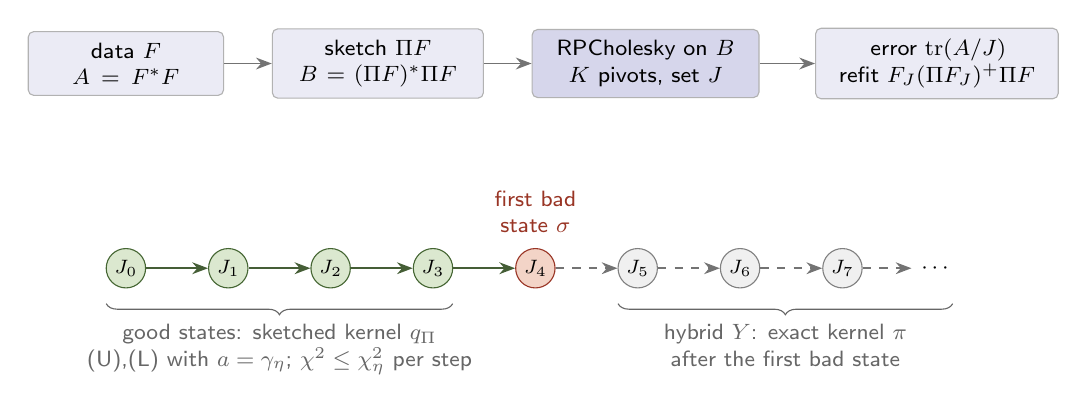
\begin{tikzpicture}[>=Stealth,font=\sffamily\footnotesize,
 box/.style={draw=black!30,rounded corners=2pt,fill=#1,align=center,inner sep=4pt},
 box/.default=black!2,
 arr/.style={->,draw=black!55,line width=.6pt}]
\node[box=NavyBlue!8,text width=2.2cm] (F) at (0,2.2) {data $F$\\ $A=F^*F$};
\node[box=NavyBlue!8,text width=2.4cm] (PF) at (3.2,2.2) {sketch $\Pi F$\\ $B=(\Pi F)^*\Pi F$};
\node[box=NavyBlue!16,text width=2.6cm] (RP) at (6.6,2.2) {RPCholesky on $B$\\ $K$ pivots, set $J$};
\node[box=NavyBlue!8,text width=2.8cm] (out) at (10.3,2.2) {error $\tr(A/J)$\\ refit $F_J(\Pi F_J)^+\Pi F$};
\draw[arr] (F)--(PF); \draw[arr] (PF)--(RP); \draw[arr] (RP)--(out);
\begin{scope}[yshift=-.4cm]
\foreach \x/\l in {0/0,1.3/1,2.6/2,3.9/3} {
 \node[circle,draw=OliveGreen!70!black,fill=OliveGreen!15,minimum size=5mm,inner sep=0] (g\l) at (\x,0) {\scriptsize$J_{\l}$};}
\node[circle,draw=BrickRed!80!black,fill=BrickRed!15,minimum size=5mm,inner sep=0] (b4) at (5.2,0) {\scriptsize$J_4$};
\foreach \x/\l in {6.5/5,7.8/6,9.1/7} {
 \node[circle,draw=black!50,fill=black!6,minimum size=5mm,inner sep=0] (e\l) at (\x,0) {\scriptsize$J_{\l}$};}
\node (dots) at (10.3,0) {$\cdots$};
\foreach \a/\b in {g0/g1,g1/g2,g2/g3,g3/b4} \draw[arr,draw=OliveGreen!60!black] (\a)--(\b);
\foreach \a/\b in {b4/e5,e5/e6,e6/e7,e7/dots} \draw[arr,dashed] (\a)--(\b);
\draw[decorate,decoration={brace,amplitude=4pt,mirror},black!60] (-.25,-.45)--(4.15,-.45)
 node[midway,below=4pt,align=center] {good states: sketched kernel $q_\Pi$\\
 (U),(L) with $a=\gamma_\eta$; $\chi^2\le\chi^2_\eta$ per step};
\draw[decorate,decoration={brace,amplitude=4pt,mirror},black!60] (6.25,-.45)--(10.5,-.45)
 node[midway,below=4pt,align=center] {hybrid $Y$: exact kernel $\pi$\\
 after the first bad state};
\node[above=2pt,text=BrickRed!80!black,align=center] at (b4.north) {first bad\\ state $\sigma$};
\end{scope}
\end{tikzpicture}
\caption{Sketched RPCholesky (top) and the analysis (bottom). The
sketched chain $X$ and the hybrid $Y$ agree up to the first bad state.
The hybrid satisfies the functional hypotheses of
Proposition~\ref{prop:functional} for every $\Pi$, so it reaches
$(1+\eps)\tau$; the two chains differ only on an event of probability
$\Pfail$, controlled by the $\chi^2$ path likelihood against exact
RPCholesky, whose states do not depend on $\Pi$.}
\label{fig:pipeline}
\end{figure}
\subsection{The main theorem}
For $r\ge2$, $0<\eps\le1$, $0<\eta\le1/4$ and $0<\beta<1$ define the
sketched count
\begin{equation}\label{eq:Ksk}
 K^{\mathrm{sk}}(r,\eps;\eta,\beta)
 =\calK_{\gamma_\eta}\Bigl(r,\eps;\ \frac{1-\beta}2,\
 \frac{H^{(4)}_{r,\beta}+r\chi^2_\eta}2\Bigr),
\end{equation}
with $\calK_a$ from~\eqref{eq:calK}. In the cooling formula the
effective moment scale is $H/(r\theta)=(H^{(4)}_{r,\beta}/r+\chi^2_\eta)/(1-\beta)$,
so the sketch adds only $\chi^2_\eta/(1-\beta)$ to it. Since $\gamma_\eta\ge0.55$
and $\chi^2_\eta\le0.101$ for $\eta\le1/4$, Corollary~\ref{cor:two-sided}'s
argument gives $K^{\mathrm{sk}}=O(r/\eps+r\Lambda_4(r))$ for fixed
$\beta$, uniformly in $\eta\le1/4$.

\begin{theorem}[Sketched RPCholesky]\label{thm:sketch}
Let $r\ge2$, $0<\eps\le1$, $0<\eta\le1/4$, $0<\beta<1$, and
$\tau=\tau_r(A)>0$. Let $K\ge K^{\mathrm{sk}}(r,\eps;\eta,\beta)$ and let
$\Pi$ be independent of the pivot randomness and have
$\MP(K+1,\ell,\eta/2)$ with $\ell\ge2$. Let $J_0,\dots,J_K$ be the
states of sketched RPCholesky and
$\Pfail=\Prob\{\calG(J_s)\text{ fails for some }s\le K\}$. Then
\begin{equation}\label{eq:sketch-main}
 \begin{aligned}
 \E\tr R_A(J_K)&\le(1+\eps)\tau+\Pfail\tr A,\\
 \Pfail&\le e^{K\chi^2_\eta/2}\sqrt{(K+1)\delta_1}\\
 &=2(K+1)\,e^{K\chi^2_\eta/2}\,2^{-\ell/2}.
 \end{aligned}
\end{equation}
The expectation is over $\Pi$ and the pivots.
\end{theorem}

\begin{proof}
\emph{Step 1: the hybrid process.} Fix $\Pi$. Drive all chains by the
same i.i.d.\ uniform variables $V_1,V_2,\dots$, independent of $\Pi$:
at step $s+1$ a chain draws its pivot from its current kernel by
inversion of the distribution function with $V_{s+1}$. The sketched
chain $X$ uses $q_\Pi(\cdot\mid J_s)$. The hybrid chain $Y$ uses
\[
 \kappa_s=\begin{cases}
 q_\Pi(\cdot\mid J^Y_s)&\text{if }\calG(J^Y_0),\dots,\calG(J^Y_s)\text{ all hold},\\
 \pi(\cdot\mid J^Y_s)&\text{otherwise.}\end{cases}
\]
Let $\sigma$ be the first $s\le K$ at which the state of $X$ is bad
($\sigma=\infty$ if there is none). At a good state with $R_A\ne0$,
$\tr R_B>0$ by~\eqref{eq:trace-comparison}, so $X$ does not stop
before $\sigma$. The kernels of $X$ and $Y$ agree at every $s<\sigma$,
so $J^X_s=J^Y_s$ for all $s\le\min\{\sigma,K\}$. Hence the event
$\{\sigma\le K\}$ is the same for both chains, its probability is
$\Pfail$, and $J^X_K=J^Y_K$ on $\{\sigma>K\}$. Since
$0\le\tr R_A(J)\le\tr A$,
\begin{equation}\label{eq:hybrid-split}
 \tr R_A(J^X_K)\le\tr R_A(J^Y_K)+\tr A\,\1\{\sigma\le K\}.
\end{equation}

\emph{Step 2: the hybrid satisfies (U) and (L) with $a=\gamma_\eta$.}
Let $\calF_k$ be generated by $\Pi$ and $V_1,\dots,V_k$. At a time $k$
with a good prefix, Lemma~\ref{lem:kernel}(a),(b) gives (U) and (L);
at all other times $Y$ uses the exact kernel, for which (U) and (L)
hold with $a=1$, hence with $a=\gamma_\eta$. Every pivot of $Y$ is
positive for $A$ (Lemma~\ref{lem:sk-residual}).

\emph{Step 3: the path likelihood.} Let $p$ denote the law of the first
$K$ pivots of exact RPCholesky on $A$; it does not depend on $\Pi$.
After exhaustion append a deterministic null transition, with likelihood
ratio one. For fixed $\Pi$, Lemma~\ref{lem:sk-residual} shows that each $\kappa_s$ is
absolutely continuous with respect to $\pi(\cdot\mid J_s)$, so the law
of the first $k$ pivots of $Y$ has density
\[
 L_k=\prod_{s<k}\frac{\kappa_s(i_s)}{\pi(i_s\mid J_s)}
\]
with respect to $p$. Under $p$, $\E_p[L_{s+1}^2\mid i_0,\dots,i_{s-1}]
=L_s^2\sum_i\kappa_s(i)^2/\pi(i\mid J_s)\le(1+\chi^2_\eta)L_s^2$, by
Lemma~\ref{lem:kernel}(c) at good-prefix states and with equality to
$L_s^2$ otherwise. Hence, for every $\Pi$ and every $k\le K$,
\begin{equation}\label{eq:L2}
 \E_pL_k^2\le(1+\chi^2_\eta)^k\le e^{k\chi^2_\eta}.
\end{equation}

\emph{Step 4: the first failure.} The event $\{\sigma\le K\}$ is a
function of $\Pi$ and of the first $K$ pivots. Therefore, by
Cauchy--Schwarz jointly in $\Pi$ and the path,
\[
 \Pfail=\E_\Pi\E_p\bigl[L_K\1\{\sigma\le K\}\bigr]
 \le\bigl(\E_\Pi\E_pL_K^2\bigr)^{1/2}
 \Bigl(\E_p\sum_{s=0}^K\Prob_\Pi\{\calG(J_s)^c\}\Bigr)^{1/2}.
\]
Under $p$ the states $J_s$ do not depend on $\Pi$ and have
$|J_s|\le s\le K$, including after exhaustion, so Lemma~\ref{lem:bad} bounds each probability in the
sum by $\delta_1$. With~\eqref{eq:L2} this gives the bound on $\Pfail$.

\emph{Step 5: the initial moment of the hybrid.} Put $\theta_0=1-\beta$.
By Step~3, Cauchy--Schwarz, \eqref{eq:L2} and Imported
Theorem~\ref{imp:four},
\begin{align*}
 \E\,P\bigl(R_A(J^Y_r)\bigr)^{\theta_0/2}
 &=\E_\Pi\E_p\bigl[L_rP(R_A(J_r))^{\theta_0/2}\bigr]\\
 &\le\bigl(\E_\Pi\E_pL_r^2\bigr)^{1/2}\bigl(\E_pP(R_A(J_r))^{\theta_0}\bigr)^{1/2}
 \le e^{(r\chi^2_\eta+H^{(4)}_{r,\beta})/2}.
\end{align*}
This is hypothesis (I) with $\theta=\theta_0/2$ and
$H=(H^{(4)}_{r,\beta}+r\chi^2_\eta)/2$.

\emph{Step 6: conclusion.} Proposition~\ref{prop:functional}, applied to
$Y$ with the filtration of Step~2, gives
$\E\tr R_A(J^Y_K)\le(1+\eps)\tau$. Taking expectations
in~\eqref{eq:hybrid-split} proves~\eqref{eq:sketch-main}.
\end{proof}

\begin{remark}[H\"older exponents]\label{rem:holder}
Step~5 may use H\"older with exponents $p\in(1,2]$ and $p/(p-1)$ in
place of Cauchy--Schwarz. Log-convexity of moments gives
$\E_pL_r^p\le(\E_pL_r^2)^{p-1}$, and the resulting hypothesis is (I)
with $\theta=\theta_0(1-1/p)$ and $H=(1-1/p)(H^{(4)}_{r,\beta}+r\chi^2_\eta)$.
The ratio $H/\theta$, which drives the cooling phase, does not depend on
$p$; the choice $p=2$ gives the largest exponent $\theta$.
\end{remark}

\begin{remark}[The determinant route]\label{rem:det-route}
Lemma~\ref{lem:likelihood} gives a second bound on the first failure
without the hybrid likelihood. On $\{\sigma=t\}$ the states
$J_0,\dots,J_{t-1}$ are good, so by~\eqref{eq:trace-comparison} the
likelihood of the first $t$ steps is at most
$(1-\eta-\eta^2)^{-t}\det G_{J_t}$. Cauchy--Schwarz in $\Pi$ gives
\[
 \Prob\{\sigma=t\}\le(1-\eta-\eta^2)^{-t}
 \sup_{|J|=t}\bigl(\E\det G_J^2\bigr)^{1/2}\delta_1^{1/2}.
\]
By AM--GM and the power-mean inequality,
$\det G_J\le(1+|\tr Z_{Q_J}|/t)^t$ and
$|\tr Z|/t\le(\tr Z^{2\ell}/t)^{1/(2\ell)}$. If $t\le\ell$, Minkowski's
inequality in $L^{2t}$ and the moment property give
$\E\det G_J^2\le\bigl(1+((K+1)/t)^{1/(2\ell)}\eta/2\bigr)^{2t}$. The
resulting bound $\Pfail\le e^{O(\eta K)}\delta_1^{1/2}$ needs
$\ell\ge K$ and pays $O(\eta)$ nats per step; the $\chi^2$ route of
Theorem~\ref{thm:sketch} pays $O(\eta^2)$ and needs no relation between
$\ell$ and $K$.
\end{remark}

\begin{remark}[Per-coordinate brackets]\label{rem:per-coordinate}
If the good event at $J$ also required $\|Z_{U}\|\le\eta$ for every
frame $U=[Q_J,u_i]$, $i\in\Sigma_J$, then the variational formula for
$(R_B)_{ii}$ would give the per-coordinate bracket
$\frac{1-\eta}{1+\eta}\pi_i\le q_i\le\frac{1+\eta}{1-\eta}\pi_i$, and
Corollary~\ref{cor:two-sided} would apply directly to the hybrid. That
event costs a union bound over up to $N$ coordinates per state, so
$\log N$ would enter the moment order $\ell$. The functional
formulation of Proposition~\ref{prop:functional} is what removes it.
\end{remark}
\subsection{Reusing the sketch for the reconstruction}
The natural output of sketched RPCholesky is the column set together
with the regression computed from the same sketch.

\begin{corollary}[Sketch reuse]\label{cor:reuse}
In the setting of Theorem~\ref{thm:sketch}, let $J=J_K$ and
$X_B=(\Pi F_J)^+\Pi F$. If $\calG(J)$ holds, then
\[
 \|F-F_JX_B\|_F^2\le\Bigl(1+\frac{\eta^2}{2(1-\eta)^2}\Bigr)\tr R_A(J).
\]
Consequently, with $\sigma$ as in the proof of Theorem~\ref{thm:sketch},
\[
 \E\bigl[\|F-F_JX_B\|_F^2\,\1\{\sigma>K\}\bigr]
 \le\Bigl(1+\frac{\eta^2}{2(1-\eta)^2}\Bigr)(1+\eps)\tau,
 \qquad \Prob\{\sigma\le K\}\le\Pfail .
\]
\end{corollary}
\begin{proof}
If $R_A(J)=0$ then $F=F_JX$ for some $X$ and $X_B=X$ because $\Pi F_J$
has full column rank (Lemma~\ref{lem:sk-residual}); the error is zero.
Otherwise write $F_J=QC$ with $Q=Q_J$ and $C$ invertible, and
$X_\star=C^{-1}Q^*F$, so that $F-F_JX_\star=E_J$. Since
$\Pi F=\Pi F_JX_\star+\Pi E_J$ and $(\Pi F_J)^+\Pi F_J=I$,
\[
 X_B-X_\star=(\Pi F_J)^+\Pi E_J,\qquad
 F_J(\Pi F_J)^+=QC\,C^{-1}(\Pi Q)^+=QG_J^{-1}Q^*\Pi^* .
\]
Hence $F-F_JX_B=E_J-QG_J^{-1}Q^*\Pi^*\Pi E_J$. The two terms are
orthogonal because $Q^*E_J=0$, so by Lemma~\ref{lem:good}(a),(d),
\[
 \|F-F_JX_B\|_F^2=\tr R_A(J)+\|G_J^{-1}Q^*\Pi^*\Pi E_J\|_F^2
 \le\tr R_A(J)+\frac{\eta^2}{2(1-\eta)^2}\tr R_A(J).
\]
For the second claim, $J^X_K=J^Y_K$ on $\{\sigma>K\}$, so
$\E[\tr R_A(J^X_K)\1\{\sigma>K\}]\le\E\tr R_A(J^Y_K)\le(1+\eps)\tau$.
\end{proof}

On the bad event the oblique refit is not controlled: $G_J$ may be
nearly singular, and $\|F-F_JX_B\|_F$ can exceed $\|F\|_F$. The
corollary is therefore a statement on an event of probability at least
$1-\Pfail$, not a bound in expectation. The exact refit
$F_JF_J^+F$ has error $\tr R_A(J)$ and inherits
Theorem~\ref{thm:sketch} in expectation, at the cost of a pass over $F$.

\subsection{SparseStack and SRHT}
We import the moment certificates of two oblivious sketches. SparseStack
is the stacked one-sparse construction used in~\cite{CEMT,EpperlyARP},
in the line of OSNAP~\cite{NN13}; the constants below are the certificate
of~\cite{SparseStack}, not a claim to have introduced that construction.
The second sketch is a two-round variant of the subsampled randomized
Hadamard transform~\cite{Tropp11}, with the certificate
of~\cite{SRHThybrid}.

\begin{imported}[{\cite[Theorem 10.6 and Appendix B.4--B.5]{SparseStack}}]\label{imp:sparsestack}
Let $d,\ell\ge2$ and $0<\eta\le1$. The fully independent real SparseStack
matrix with $s_\Pi=\lceil(17/2)(2\ell+1)/\eta\rceil$ nonzeros per column,
$b=\lceil81(d+2\ell+1)/(\eta^2s_\Pi)\rceil$ rows per block and
$m=s_\Pi b$ rows satisfies $\E\tr Z_U^{2\ell}<d(\eta/2)^{2\ell}$ for every
real isometry $U$ with $d$ columns. Moreover $s_\Pi<26.5\ell/\eta$ and
$m<179(d+\ell)/\eta^2$.
\end{imported}

\begin{imported}[{\cite[Equation (5.6) and Theorem 1.1]{SRHThybrid}}]\label{imp:srht}
Let $n\ge D$ be a power of two, pad $F$ with zero rows to $n$ rows, and
let $\Pi=\sqrt{n/M}\,R_TW_nD_yW_nD_x$ be the two-round Walsh transform, where $W_n$ is the normalized (unitary) Walsh--Hadamard matrix,
with independent Rademacher diagonals $D_x,D_y$ and a uniform
$M$-subset $T$ of rows, with $1\le M\le n$. If
$M\ge216(d+12\ell^2)/\eta^2$, or $M=n$, then
$\E\tr Z_U^{2\ell}\le d(\eta/2)^{2\ell}$ for every complex isometry $U$
with $d$ columns.
\end{imported}

The case $M=n$ is a full unitary transform, so its distortion is exactly
zero. The moment bound is then valid for every $d$ and $\ell$ without
the displayed row threshold.

By Remark~\ref{rem:MP}(i) both certificates give
$\MP(d,\ell,\eta/2)$. For complex data and the real SparseStack,
Remark~\ref{rem:MP}(ii) applies with $2d$ in place of $d$.

\begin{corollary}[Explicit sketch sizes]\label{cor:instances}
Let $r\ge2$, $0<\eps\le1$, $0<\eta\le1/4$, $0<\beta<1$, let
$K\ge K^{\mathrm{sk}}(r,\eps/2;\eta,\beta)$, and choose
\begin{equation}\label{eq:ell-choice}
 \ell\ge\max\Bigl\{2,\ 2\log_2\frac{4(K+1)\tr A}{\eps\tau_r(A)}
 +\frac{K\chi^2_\eta}{\log2}\Bigr\}.
\end{equation}
If $\Pi$ is the SparseStack of Imported Theorem~\ref{imp:sparsestack}
with $d=K+1$ (real $F$), or the two-round SRHT of Imported
Theorem~\ref{imp:srht} with $d=K+1$, then sketched RPCholesky with $K$
pivots satisfies $\E\tr R_A(J_K)\le(1+\eps)\tau_r(A)$. The sketch sizes
are
\[
 m_{\mathrm{SS}}<\frac{179(K+1+\ell)}{\eta^2}
 =O\Bigl(\frac{K+\log(\tr A/(\eps\tau_r))}{\eta^2}\Bigr),\qquad
 s_\Pi=O\Bigl(K\eta+\frac{\log(K\tr A/(\eps\tau_r))}\eta\Bigr),
\]
and
\[
 M_{\mathrm{SRHT}}=\min\Bigl\{n,\Bigl\lceil\frac{216(K+1+12\ell^2)}{\eta^2}\Bigr\rceil\Bigr\}
 =O\Bigl(\frac K{\eta^2}+K^2\eta^2
 +\frac{\log^2(K\tr A/(\eps\tau_r))}{\eta^2}\Bigr).
\]
\end{corollary}
\begin{proof}
By~\eqref{eq:ell-choice},
$2(K+1)e^{K\chi^2_\eta/2}2^{-\ell/2}\le\eps\tau_r/(2\tr A)$, so
Theorem~\ref{thm:sketch} with $\eps/2$ gives
$(1+\eps/2)\tau_r+\eps\tau_r/2$. The size bounds follow from
$\ell=O(K\eta^2+\log(K\tr A/(\eps\tau_r)))$, $\chi^2_\eta\le2\eta^2$ for
$\eta\le1/4$, and $\log K\le K$.
\end{proof}

For fixed $\eta$ the SparseStack row count is linear in the pivot budget
$K$ plus a logarithm of $\tr A/(\eps\tau_r)$; it is independent of $N$,
of $D$ and of the rank of $F$. Two costs should be stated plainly. The
moment order grows linearly in $K\eta^2$, so the column sparsity
$s_\Pi$ grows like $K\eta$: the sketches covered by the theorem are
relatively dense. For SRHT the quadratic moment term makes the row count
at least of order $K^2\eta^2$; minimizing over $\eta$ gives
$\eta\asymp K^{-1/4}$ and $M=O(K^{3/2})$ up to logarithms, while the
pivot count then approaches the exact one, since
$1-\gamma_\eta=O(K^{-1/4})$. Table~\ref{tab:sk-params} evaluates these
formulas; the proved constants are large ($m/K$ of order $10^3$--$10^4$
for SparseStack), and the experiments of Section~\ref{sec:numerics}
show exact-RP behaviour already at $m=2K$.

\subsection{Why a pure change of measure is not enough}\label{sec:chi-only}
A direct transfer compares the terminal errors under the sketched path
law $Q$ and the exact law $P$. For $f=\tr R_A(J_K)$,
\[
 |\E_Qf-\E_Pf|\le\sqrt{\chi^2(Q\Vert P)}\,\sqrt{\operatorname{Var}_Pf}.
\]
Even in the favourable case $\chi^2(Q\Vert P)\lesssim K/m$ and
$\operatorname{Var}_Pf=O(\tau_r^2)$, this perturbation is of order
$\sqrt{K/m}\,\tau_r$, and this variance estimate certifies an error
allowance $\eps\tau_r$ when
$m\gtrsim K/\eps^2$. At $r=100$ and $\eps=0.1$ this is
$K/\eps^2=1.85\times10^5$ against the pivot count $K=1852$.

The comparison with Corollary~\ref{cor:instances} is one of scaling in
$\eps$. With $K\asymp r/\eps$, a $\chi^2$-only variance bound gives a sufficient scale of order
$r/\eps^3$ rows, while Corollary~\ref{cor:instances} needs of order
$r/\eps$ rows at fixed $\eta$. The proved constant in front of the latter
is large ($m_{\mathrm{SS}}/K\approx1.7\cdot10^3$ at $\eta=1/4$,
Table~\ref{tab:sk-params}), and the heuristic $K/\eps^2$ carries no
constant at all, so in absolute numbers the gain appears only for small
$\eps$; the point of Theorem~\ref{thm:sketch} is that the accuracy
parameter never enters the sketch distortion.

Theorem~\ref{thm:sketch} uses the likelihood only in two places where a
constant factor is harmless. In the initial moment, the factor
$e^{r\chi^2_\eta/2}$ is absorbed into $H$, exactly as the factor $a^{-r}$
is absorbed under a two-sided bracket. In the failure probability, the
factor $e^{K\chi^2_\eta/2}$ multiplies the exponentially small
$\sqrt{(K+1)\delta_1}$ and is paid by $\ell=O(K\eta^2)$ extra moment
orders. The accuracy itself comes from the drift inequalities (U) and
(L), which hold conditionally on every good history with the constant
$\gamma_\eta$. A constant $\gamma_\eta<1$ costs a constant factor in the
pivot count, not a loss in the attained accuracy. So the distortion
$\eta$ can stay fixed while $\eps\to0$, and $\eps$ enters the sketch
size only through $K$ and $\log(1/\eps)$.

What is proved is exactly~\eqref{eq:sketch-main}: an expectation bound
with the additive term $\Pfail\tr A$. The proof retains this term because
it controls a failed history only by $\tr A$. Making that contribution
smaller than $\eps\tau_r$ is why $\log(\tr A/\tau_r)$ enters the moment order.
It does not enter the pivot count.
\section{Fixed-dictionary frame selection by an RP gate}\label{sec:gate}
A subspace embedding guarantee is proved for a subspace fixed before the
sketch is drawn. When the subspace is selected with the help of the
sketch, a union bound over all candidates is the default price. A
selection rule with a controlled likelihood pays much less. This section
records the pointwise price of one such rule and compares it with a
R\'enyi price derived from Imported Theorem~\ref{imp:four}. The factorial
comparison is the adaptive-sampling argument of Deshpande and
Vempala~\cite{DV}; the factor $\Lambda_C$ keeps the residual-trace
denominators of that argument, which the bound $k!$ discards.

Fix an isometry $V\in\C^{N\times k}$ and, for every $k$-subset
$J\subseteq[N]$, a target isometry $U_J$, all before drawing a sketch
$S$. Let $C(S)$ be a measurable positive definite $k\times k$ matrix.
After drawing $S$, run $k$ steps of exact RPCholesky on $VC(S)V^*$ with
fresh randomness, and release only the unordered terminal set $J$. The
reference law
\[
 \nu_V(J)=|\det V_J|^2,
\]
where $V_J$ is the $k\times k$ submatrix of rows $J$, is a probability
distribution by the Cauchy--Binet formula and does not depend on $S$.

\begin{theorem}[Pointwise gate price]\label{thm:gate}
For eigenvalues $\lambda_1\ge\cdots\ge\lambda_k>0$ of $C$ put
\[
 \tau_j(C)=\sum_{i>j}\lambda_i,\qquad
 \Lambda_C=\frac{k!\,\det C}{\prod_{j=0}^{k-1}\tau_j(C)} .
\]
Conditionally on $S$, the released law satisfies
$\mu_{C(S)}(J)\le\Lambda_{C(S)}\nu_V(J)$, and $1\le\Lambda_C\le k!$.
Suppose each fixed $U_J$ fails for the sketch with probability at most
$\delta_0$. If $\Lambda_{C(S)}\le\bar\Lambda$ almost surely, then the
selected $U_J$ fails with probability at most $\bar\Lambda\delta_0$. In
particular $\delta_0=\delta/k!$ always suffices for failure probability
$\delta$.
\end{theorem}
\begin{proof}
The matrix $M=VCV^*$ has rank $k$ and the same nonzero eigenvalues as
$C$. For an ordered pivot sequence with set $J$, Lemma~\ref{lem:path}
gives the product of pivots $\det M_{JJ}=\det(V_JCV_J^*)=\det C\,|\det V_J|^2$.
After $j$ pivots the residual trace is at least $\tau_j(M)=\tau_j(C)$
by Lemma~\ref{lem:order}. So each ordered path has probability at most
$\det C\,\nu_V(J)/\prod_{j<k}\tau_j(C)$, and summing over the $k!$
orders gives $\mu_C(J)\le\Lambda_C\nu_V(J)$. Moreover
$\lambda_{j+1}\le\tau_j(C)\le(k-j)\lambda_{j+1}$, and multiplying over
$j$ gives $1\le\Lambda_C\le k!$. Let $\mathcal B_J$ be the failure event
of the fixed target $U_J$. Conditionally on $S$ and then on average,
\[
 \Prob\{\mathcal B_J\text{ for the selected }J\}
 =\E_S\sum_J\mu_{C(S)}(J)\1_{\mathcal B_J}(S)
 \le\bar\Lambda\sum_J\nu_V(J)\Prob_S(\mathcal B_J)\le\bar\Lambda\delta_0 .
\]
The weights $\nu_V$ and the targets $U_J$ were fixed before $S$, so only
fixed-subspace guarantees are used.
\end{proof}

A flat $C$ gives $\Lambda_C=1$. For a spike $C=I+\vartheta uu^*$ with
$\|u\|=1$, the eigenvalues are $1+\vartheta$ and $k-1$ ones, so
$\tau_0=k+\vartheta$, $\tau_j=k-j$ for $j\ge1$, and
\[
 \Lambda_C=\frac{k!\,(1+\vartheta)}{(k+\vartheta)(k-1)!}
 =\frac{k(1+\vartheta)}{k+\vartheta}\le\min\{k,1+\vartheta\}.
\]
More generally, partition the ordered eigenvalues into contiguous bands
of sizes $n_1,\dots,n_L$ with largest-to-smallest ratios
$\rho_1,\dots,\rho_L$. Bounding each $\tau_j(C)$ from below by the
remaining eigenvalues of the band of $\lambda_{j+1}$, and $\det C$ from
above by the band maxima, gives
\begin{equation}\label{eq:bands}
 \Lambda_C\le\min\Bigl\{k!,\ \frac{k!}{\prod_\ell n_\ell!}\prod_\ell\rho_\ell^{n_\ell}\Bigr\}.
\end{equation}
The bound $\bar\Lambda$ must hold uniformly over the permitted $C(S)$;
inserting the observed $\Lambda_{C(S)}$ into a failure budget chosen after
seeing $S$ is not covered. Nor does the argument cover a
sketch-dependent frame $V(S)$, partial-rank stopping, or releasing the
pivot order.

\begin{proposition}[R\'enyi gate price]\label{prop:renyi-gate}
Let $k\ge2$. For every $p>1$, without any assumption on $C(S)$, the
selected $U_J$ fails with probability at most
\[
 e^{B_{k,1/p}}\,2^{k/p}\,a_k\,\delta_0^{1-1/p}.
\]
Consequently failure probability $\delta$ is guaranteed by
\begin{equation}\label{eq:renyi-delta0}
 \log\frac1{\delta_0}=\frac p{p-1}\Bigl[\log\frac1\delta+B_{k,1/p}
 +\frac kp\log2+\log a_k\Bigr],
\end{equation}
optimized over $p$, while the pointwise price of
Theorem~\ref{thm:gate} is $\log(1/\delta_0)=\log(1/\delta)+\log k!$.
\end{proposition}
\begin{proof}
For $M=VC(S)V^*$ with $r=k$, the volume-sampling law is
$\nu_k(J)=\det M_{JJ}/e_k(M)=|\det V_J|^2=\nu_V(J)$, because
$e_k(M)=\det C$. Imported Theorem~\ref{imp:four} with $\beta=1/p$ gives
$\sum_J\nu_V(J)L(J)^p\le e^{pB_{k,1/p}}2^ka_k^p$ for $L=\mu_{C(S)}/\nu_V$,
uniformly in $S$. H\"older's inequality in the joint law of $S$ and
$J\sim\nu_V$ gives
\[
 \E_S\sum_J\nu_V(J)L(J)\1_{\mathcal B_J}(S)
 \le\Bigl(\E_S\sum_J\nu_VL^p\Bigr)^{1/p}
 \Bigl(\sum_J\nu_V(J)\Prob_S(\mathcal B_J)\Bigr)^{1-1/p},
\]
which is the stated bound.
\end{proof}

\paragraph{When each price wins.}
The pointwise exponent is $\log k!=k\log k-k+O(\log k)$. The R\'enyi
exponent is $k[1+\log b_k+O(1)]$ for fixed $p$, with
$b_k\sim\log\log k$, plus the factor $p/(p-1)$. For small $k$ the
constants dominate and $k!$ is better; for large $k$ the R\'enyi price
wins by a factor growing like $\log k/\log\log\log k$. At $\delta=0.01$,
exact evaluation of~\eqref{eq:renyi-delta0} over $p$ shows that the
R\'enyi price first beats $k!$ at $k=128$ (exponents $500.1$ against
$501.0$, at $p\approx6.8$); at $\delta=10^{-6}$ the crossover is $k=129$.
At $k=10$ the R\'enyi exponent is $38.5$ against $19.7$; at $k=1000$ it
is $3975$ against $5917$. When a spectral certificate~\eqref{eq:bands}
is available, it usually beats both at small $k$; the spike example
gives $\Lambda_C\le k$. Section~\ref{sec:numerics} converts these prices
into SparseStack row counts.
\section{Restarts: unions of independent chains}\label{sec:restart}
The initial moment in Imported Theorem~\ref{imp:four} is a fractional
moment of a determinant, and the conversion spends
$O(r\Lambda_4(r))$ pivots turning it into a first moment of the trace.
The first moment of the trace after $r$ pivots can be exponentially
large in $r$ on inputs whose fractional moments are close to their
minimum; the family below is an example. Independent restarts convert a
fractional moment of the trace into a first moment directly.

\begin{theorem}[Union amplification]\label{thm:restart}
Let $S_1,\dots,S_m$ be the unordered pivot sets of $m$ independent runs
of exact RPCholesky with $k$ pivots each on $A$, let $S=\bigcup_jS_j$, and
let $T=\tr(A/S_1)$. If $0<\theta\le1$ and $m\ge1/\theta$, then
\[
 \E\tr(A/S)\le\bigl(\E T^\theta\bigr)^{1/\theta}.
\]
\end{theorem}
\begin{proof}
For $S_j\subseteq S$ the residual $A/S$ is obtained from $A/S_j$ by
further Schur complementation, skipping any zero residual column. Thus $A/S\preceq A/S_j$
(Lemma~\ref{lem:order}). Hence, with $T_j=\tr(A/S_j)$,
\[
 \tr(A/S)\le\min_jT_j\le\prod_{j=1}^mT_j^{1/m}.
\]
Independence is used at this point, and only at this point:
\[
 \E\prod_{j=1}^mT_j^{1/m}=(\E T^{1/m})^m.
\]
Since $1/m\le\theta$, monotonicity of $L^p$ norms completes the argument:
\[
 (\E T^{1/m})^m\le(\E T^\theta)^{1/\theta}.
\]
\end{proof}

The union needs no validation step: pivoting on the union dominates
every individual run, whichever of them happens to be best.

\begin{corollary}[A conditional $O(r/\eps)$ restart variant]\label{cor:restart}
Suppose that for constants $c>0$, $0<\theta\le1$ and $\kappa\ge1$, exact
RPCholesky satisfies the fractional warm start
\begin{equation}\label{eq:warm}
 \E\Bigl(\frac{\tr R_{\lceil cr\rceil}}{\tau_r(A)}\Bigr)^\theta\le\kappa
\end{equation}
for the input $A$ and rank $r$ with $\tau_r(A)>0$. Run
$m=\lceil1/\theta\rceil$ independent chains of $\lceil cr\rceil$ pivots,
pivot on the union $S$, and continue exact RPCholesky from $A/S$ for
\[
 n'=\Bigl\lceil r\Bigl(\frac1\eps+\log\frac1\eps+\frac{\log\kappa}\theta\Bigr)\Bigr\rceil
\]
further pivots. The resulting residual has expected trace at most
$(1+\eps)\tau_r(A)$, and the total number of columns is at most
$\lceil1/\theta\rceil\lceil cr\rceil+n'=O(r/\eps)$ for fixed
$c,\theta,\kappa$.
\end{corollary}
\begin{proof}
Theorem~\ref{thm:restart} gives $\E\tr(A/S)\le\kappa^{1/\theta}\tau$.
The continuation is exact RPCholesky on $A/S\preceq A$, so
every later residual $R$ satisfies $\tau_r(R)\le\tau$, and (L) holds
with $a=1$.
Let $u_0=\E\tr(A/S)/\tau-1$. If $u_0\le\eps$, no continuation is
needed. Otherwise $u_0>\eps>0$ and $u_0<\kappa^{1/\theta}$, so
$F(u_0)>-\theta^{-1}\log\kappa$. Lemma~\ref{lem:scalar}, applied to
the means, then needs at most $r(F(\eps)-F(u_0))\le n'$ steps.
\end{proof}

Whether~\eqref{eq:warm} holds uniformly over inputs is open
(Conjecture~\ref{conj:warm}). It follows from a first-moment warm start
by Jensen's inequality, but it is much weaker, as the following family
shows.

\paragraph{The scale-separated family.}
Let $n=r+1$, $0<h<1$, $\epsilon=h^{n^2}$, $D=\diag(1,\epsilon,\dots,
\epsilon^{r-1},\epsilon^r)$, and let $L$ be unit lower triangular with
$L_{ab}=h^b/(a+b)$ for $a>b$. Put $A=LDL^*$; then
$\tau_r(A)=\lambda_{\min}(A)$. We enumerated all RPCholesky histories of
$r$ pivots by exhaustive enumeration at $4096$-bit precision, for $r=2,3,4$ and
$h\in\{10^{-2},10^{-3}\}$ (Table~\ref{tab:det01}). The first moment
$\E T_r/\tau$ is within $0.01\%$ of $2^r$, while the square-root moment
$\E(T_r/\tau)^{1/2}$ lies between $1.00016$ and $1.00254$, and the union
of two independent chains has $\E\tr(A/S)/\tau=1+O(10^{-9})$. The large
first moment comes from rare histories that pick a lower-scale
coordinate early; a fractional moment discounts them. This is numerical
evidence, not a proof, that~\eqref{eq:warm} with $\theta=1/2$ and
$\kappa$ close to one is compatible with an exponentially large first
moment.

\begin{table}[ht]
\centering
\begin{tabular}{rrrrrr}
\toprule
$r$ & $h$ & $\E T_r/\tau$ & $\E(T_r/\tau)^{1/2}$ & $\E(T_r/\tau)^{1/4}$ & union of two: $\E\tr(A/S)/\tau$\\
\midrule
2 & $10^{-2}$ & 4.0000 & 1.00254 & 1.00012 & $1+4.0\cdot10^{-10}$\\
2 & $10^{-3}$ & 4.0000 & 1.00025 & 1.000004 & $1+4\cdot10^{-14}$\\
3 & $10^{-2}$ & 7.9996 & 1.00203 & 1.00009 & $1+2.8\cdot10^{-10}$\\
3 & $10^{-3}$ & 8.0000 & 1.00020 & 1.000003 & $1+3\cdot10^{-14}$\\
4 & $10^{-2}$ & 15.998 & 1.00169 & 1.00007 & $1+2.0\cdot10^{-10}$\\
4 & $10^{-3}$ & 16.000 & 1.00017 & 1.000002 & $1+2\cdot10^{-14}$\\
\bottomrule
\end{tabular}
\caption{Exact enumeration on the scale-separated family (numerical).
Here $T_r=\tr R_r$ and $\tau=\tau_r(A)$. For $n=r+1$ two chains whose
sets differ already exhaust $A$, so the union column is
$\sum_S\mu_r(S)^2\,\tr(A/S)/\tau$.}
\label{tab:det01}
\end{table}
\section{Numerical illustrations}\label{sec:numerics}
The original experiments use Julia; their sources and recorded outputs
are supplied in the repository's \href{https://github.com/DiarHaidary/Results/tree/main/manuscripts/06-Robust-Sketched-RPCholesky/checks}{checks directory}.
Pivot counts evaluate the proved formulas. The trichotomy curves sum
the full state distribution by dynamic programming, subject only to
floating-point arithmetic. The sketching experiments are Monte Carlo
estimates, not certificates of the good event. The independent review
checks and the audit record distinguish rerun calculations from retained
experimental outputs.

\subsection{Robust pivot counts}
Table~\ref{tab:Ka} evaluates $K_a$ of Corollary~\ref{cor:two-sided}
with $\theta=1-\beta$, $H=H^{(4)}_{r,\beta}$, and $\beta$ minimized over a
grid of step $10^{-3}$. At $a=1$ the counts reproduce the four-logarithm
counts of~\cite{RA01}. The growth in $a$ is close to $1/a$, and it is
concentrated in the accuracy phase: at $r=1000$, $\eps=0.1$ the four
phases are $(1000,1104,2052,14389)$ at $a=1$ and
$(1000,1127,2482,30389)$ at $a=1/2$.

\begin{table}[ht]
\centering
\begin{tabular}{rrrrrr}
\toprule
$r$ & $\eps$ & $a=1$ & $a=0.8$ & $a=0.5$ & $a=0.25$\\
\midrule
10 & 1 & 71 & 85 & 123 & 235\\
10 & 0.1 & 185 & 226 & 349 & 687\\
100 & 1 & 722 & 848 & 1237 & 2360\\
100 & 0.1 & 1852 & 2261 & 3497 & 6881\\
1000 & 1 & 7243 & 8497 & 12393 & 23610\\
1000 & 0.1 & 18545 & 22625 & 34998 & 68821\\
\bottomrule
\end{tabular}
\caption{Two-sided robust counts $K_a$ (evaluated formula).}
\label{tab:Ka}
\end{table}

\subsection{The trichotomy on the diagonal family}
Take $A=\diag(\Theta I_r,I_m)$ with $m=4000$, $a=1/2$ and
$\Theta=(m-1000)(1-a)/(ar)$, the construction of Theorem~\ref{thm:upper}(b)
for the budget $1000$. The state is the pair $(h,b)$ of remaining heads
and tails, so the law of the residual can be propagated exactly. We
compare exact RPCholesky with three adversaries that, at every state,
give the heads the least total mass their constraint allows (uniformly
within heads and within tails): two-sided,
$q_{\mathrm{head}}=\max\{a\pi_{\mathrm{head}},1-\pi_{\mathrm{tail}}/a\}$;
lower-only, $q_{\mathrm{head}}=a\pi_{\mathrm{head}}$; upper-only,
$q_{\mathrm{head}}=\max\{0,1-\pi_{\mathrm{tail}}/a\}$.
Figure~\ref{fig:tri-curves} shows $\E\tr R_K/\tau_r(A)$.

\begin{figure}[ht]
\centering
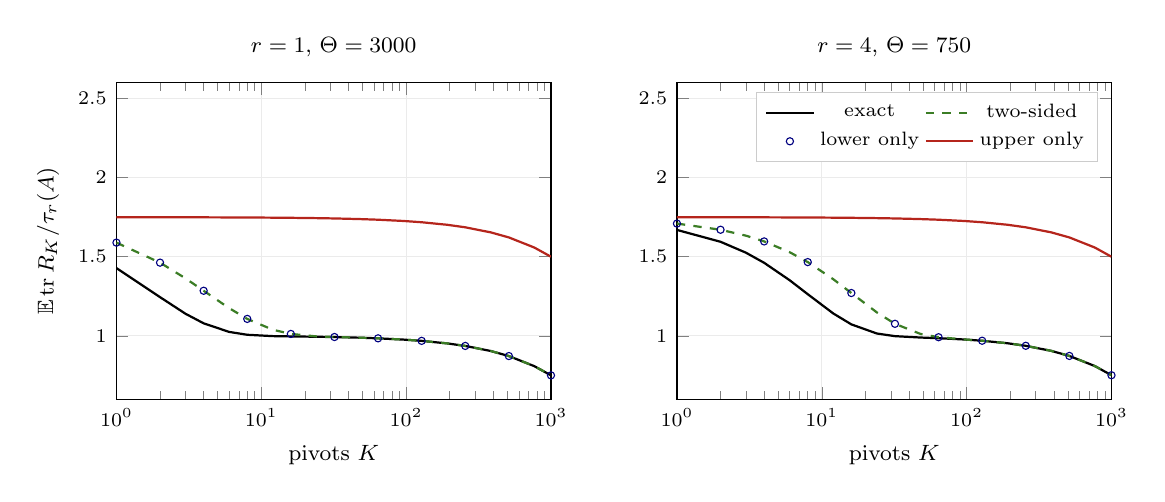
\begin{tikzpicture}
\begin{groupplot}[group style={group size=2 by 1,horizontal sep=1.6cm},
 width=7.1cm,height=5.6cm,xmode=log,xmin=1,xmax=1000,ymin=0.6,ymax=2.6,
 xlabel={pivots $K$},grid=major,grid style={black!8},
 tick label style={font=\scriptsize},label style={font=\footnotesize},
 title style={font=\footnotesize},
 legend columns=2,
 legend style={font=\scriptsize,draw=black!20,at={(0.97,0.97)},anchor=north east}]
\nextgroupplot[title={$r=1$, $\Theta=3000$},ylabel={$\E\tr R_K/\tau_r(A)$}]
\addplot[black,thick] coordinates {(1,1.4284)(2,1.2445)(3,1.1394)(4,1.0791)(6,1.0248)(8,1.0067)(12,0.9982)(16,0.9963)(24,0.9943)(32,0.9923)(48,0.9883)(64,0.9842)(96,0.9762)(128,0.9682)(192,0.9522)(256,0.9362)(384,0.9042)(512,0.8722)(768,0.8082)(1000,0.7502)};
\addplot[OliveGreen,thick,dashed] coordinates {(1,1.5891)(2,1.4626)(3,1.3631)(4,1.2849)(6,1.1750)(8,1.1070)(12,1.0386)(16,1.0120)(24,0.9965)(32,0.9926)(48,0.9883)(64,0.9843)(96,0.9763)(128,0.9683)(192,0.9522)(256,0.9362)(384,0.9042)(512,0.8722)(768,0.8082)(1000,0.7502)};
\addplot[NavyBlue,only marks,mark=o,mark size=1.3pt] coordinates {(1,1.5891)(2,1.4626)(4,1.2849)(8,1.1070)(16,1.0120)(32,0.9926)(64,0.9843)(128,0.9683)(256,0.9362)(512,0.8722)(1000,0.7502)};
\addplot[BrickRed,thick] coordinates {(1,1.7497)(2,1.7495)(3,1.7492)(4,1.7490)(6,1.7485)(8,1.7480)(12,1.7470)(16,1.7460)(24,1.7440)(32,1.7420)(48,1.7380)(64,1.7340)(96,1.7260)(128,1.7180)(192,1.7020)(256,1.6860)(384,1.6540)(512,1.6220)(768,1.5580)(1000,1.5000)};
\nextgroupplot[title={$r=4$, $\Theta=750$}]
\addplot[black,thick] coordinates {(1,1.6695)(2,1.5945)(3,1.5252)(4,1.4616)(6,1.3515)(8,1.2632)(12,1.1415)(16,1.0724)(24,1.0147)(32,0.9980)(48,0.9893)(64,0.9850)(96,0.9770)(128,0.9690)(192,0.9530)(256,0.9370)(384,0.9050)(512,0.8730)(768,0.8090)(1000,0.7510)};
\addplot[OliveGreen,thick,dashed] coordinates {(1,1.7096)(2,1.6706)(3,1.6330)(4,1.5968)(6,1.5287)(8,1.4662)(12,1.3580)(16,1.2706)(24,1.1481)(32,1.0760)(48,1.0121)(64,0.9912)(96,0.9774)(128,0.9690)(192,0.9530)(256,0.9370)(384,0.9050)(512,0.8730)(768,0.8090)(1000,0.7510)};
\addplot[NavyBlue,only marks,mark=o,mark size=1.3pt] coordinates {(1,1.7096)(2,1.6706)(4,1.5968)(8,1.4662)(16,1.2706)(32,1.0760)(64,0.9912)(128,0.9690)(256,0.9370)(512,0.8730)(1000,0.7510)};
\addplot[BrickRed,thick] coordinates {(1,1.7497)(2,1.7495)(3,1.7492)(4,1.7490)(6,1.7485)(8,1.7480)(12,1.7470)(16,1.7460)(24,1.7440)(32,1.7420)(48,1.7380)(64,1.7340)(96,1.7260)(128,1.7180)(192,1.7020)(256,1.6860)(384,1.6540)(512,1.6220)(768,1.5580)(1000,1.5000)};
\legend{exact,two-sided,lower only,upper only}
\end{groupplot}
\end{tikzpicture}
\caption{Exact expectations on $\diag(\Theta I_r,I_{4000})$ with $a=1/2$ and
$\Theta=3000/r$. The two-sided and lower-only adversaries coincide on this
family and merge with exact RPCholesky after a few dozen pivots. The
upper-only adversary never touches a head; its error is
$(r\Theta+m-K)/m$, which equals the floor $(1-K/m)/a=1.5$ at $K=1000$.}
\label{fig:tri-curves}
\end{figure}

On this family the lower-only adversary has the same head mass as the
two-sided one, because the upper constraint on the tails never binds
for the two-sided adversary here; the two curves coincide to all printed
digits. Both merge with exact RPCholesky after a few dozen ($r=1$) and
about $100$ ($r=4$) pivots, while the upper-only curve stays above $1.5$ throughout, in
agreement with Theorem~\ref{thm:upper}(b). The same programs with a very
large head, $\Theta=10^6$ and $10^8$, show the two-sided adversary paying
only in the first $r$ pivots: for $r=8$, $m=2000$ the error at $K=8$ is
$6.44\tau$ against $3.72\tau$ for exact RPCholesky, and from $K=16$ on
the two agree.
\subsection{Sketched versus exact RPCholesky}
\paragraph{Error and reuse.}
Let $D=300$, $N=400$, $r=5$, and $F=U\Sigma V^*+T$, where $U,V$ are
random orthonormal $5$-frames, $\Sigma=\diag(10^3/j)_{j\le5}$, and $T$
is a normalized product of Gaussian $300\times200$ and $200\times400$
matrices. Then $\tr A/\tau_5(A)=5051$. We compare exact RPCholesky
with sketched RPCholesky for a Gaussian sketch and a SparseStack sketch
with $4$ nonzeros per column, over $150$ trials each
(Table~\ref{tab:sk-err}). The reuse column is the median of
$\|F-F_JX_B\|_F^2/\tr R_A(J)$.

\begin{table}[ht]
\centering
\begin{tabular}{rrcrrrr}
\toprule
& & exact & \multicolumn{2}{c}{Gaussian} & \multicolumn{2}{c}{SparseStack}\\
\cmidrule(lr){4-5}\cmidrule(lr){6-7}
$k$ & $m$ & $\E\tr R/\tau$ & $\E\tr R_A/\tau$ & reuse & $\E\tr R_A/\tau$ & reuse\\
\midrule
10 & 10 & 1.550 & 1.604 & 9.02 & 1.909 & 7.71\\
10 & 20 &       & 1.571 & 1.96 & 1.559 & 1.96\\
10 & 40 &       & 1.541 & 1.34 & 1.545 & 1.32\\
20 & 20 & 1.071 & 1.067 & 12.2 & 1.064 & 12.5\\
20 & 40 &       & 1.062 & 1.97 & 1.066 & 1.97\\
20 & 80 &       & 1.067 & 1.33 & 1.065 & 1.33\\
40 & 40 & 0.744 & 0.745 & 24.8 & 0.745 & 23.4\\
40 & 80 &       & 0.745 & 1.98 & 0.746 & 1.98\\
40 & 160 &      & 0.744 & 1.33 & 0.743 & 1.33\\
\bottomrule
\end{tabular}
\caption{Sketched versus exact RPCholesky (numerical, $150$ trials).
The pivot errors are close to those of exact RPCholesky from $m=2k$
on; the same-sketch reuse ratios are compared with the fixed-design
Gaussian benchmark $1+k/(m-k-1)$.}
\label{tab:sk-err}
\end{table}

The observed pivot errors are close to those of exact RPCholesky from
$m=2k$ on, and even at $m=k$ for $k\ge20$. The reuse medians are about
$1.96$--$1.98$ at $m=2k$ and $1.33$ at $m=4k$.
For a fixed rank-$k$ design and an independent real Gaussian sketch,
the mean factor is $1+k/(m-k-1)$ when $m>k+1$, by the Gaussian
pseudoinverse moment~\cite[Proposition 10.2]{HMT}. Its large-$k$ limits
at these two aspect ratios are $2$ and $4/3$. This is a comparison
benchmark, not an exact identity for adaptive same-sketch selection or
for medians.
At $m=k$ the refit is unstable, as the
bad-event discussion after Corollary~\ref{cor:reuse} predicts (maxima
up to $1397$ over the trials).

\paragraph{The quantities in the proof.}
To see the good-event quantities along actual paths, let $D=2000$,
$N=400$, $r=5$ with the same construction ($\tr A/\tau_5=752$), and use
SparseStack with $8$ nonzeros per column ($100$ trials). Along each
sketched path we record the largest trace distortion
$|\tr R_B/\tr R_A-1|$, the largest per-step $\chi^2$ divergence
$\sum_iq_i^2/\pi_i-1$ of Lemma~\ref{lem:kernel}(c), and the accumulated
log-likelihood cost $\sum_s\log(1+\chi^2_s)$
(Table~\ref{tab:sk-path}; Gaussian sketches give similar medians for
these quantities).

\begin{table}[ht]
\centering
\begin{tabular}{rrrrrrr}
\toprule
$K$ & $m$ & $\E\tr R_A/\tau$ & $\max_s|\tr R_B/\tr R_A-1|$ & $\max_s\chi^2_s$ & $\sum_s\log(1+\chi^2_s)$ & reuse\\
\midrule
20 & 40 & 1.114 & 0.487 & 0.095 & 1.10 & 1.97\\
20 & 80 & 1.119 & 0.250 & 0.033 & 0.46 & 1.33\\
20 & 160 & 1.118 & 0.135 & 0.014 & 0.21 & 1.14\\
40 & 80 & 0.831 & 0.493 & 0.048 & 1.23 & 1.98\\
40 & 160 & 0.829 & 0.246 & 0.017 & 0.51 & 1.33\\
40 & 320 & 0.831 & 0.126 & 0.008 & 0.24 & 1.14\\
\bottomrule
\end{tabular}
\caption{Path quantities for SparseStack sketches (numerical, medians
over $100$ trials). Exact RPCholesky gives $\E\tr R/\tau=1.118$ at
$K=20$ and $0.830$ at $K=40$.}
\label{tab:sk-path}
\end{table}

The trace distortion scales like $\sqrt{K/m}$, as a subspace embedding
of dimension $K$ would. The per-step $\chi^2$ is smaller than the
square of the trace distortion, and the accumulated cost stays of order
one. This is the mechanism of Theorem~\ref{thm:sketch}: the likelihood
cost grows like $K\chi^2$ with $\chi^2$ quadratic in the distortion,
while the error is controlled by drifts that tolerate a constant
distortion.

\subsection{Proved sketch sizes}
Table~\ref{tab:sk-params} evaluates Corollary~\ref{cor:instances} with
$\tr A/\tau_r=10^6$, $\beta$ optimized, and $\ell$ the smallest integer
allowed by~\eqref{eq:ell-choice}. The listed SRHT values are uncapped
sufficient thresholds; when a threshold exceeds the padded ambient
dimension $n$, all $n$ rows are used and the transform is exact.
The proved thresholds are far above the
experimental ones; they are a scope statement: linear in $K$ for
SparseStack at fixed $\eta$, with no dependence on $N$ or $D$.

\begin{table}[ht]
\centering
\begin{tabular}{rrrrrrrr}
\toprule
$r$ & $\eps$ & $\eta$ & $K_4(r,\eps)$ & $K^{\mathrm{sk}}(r,\eps/2)$ & $\ell$ & $m_{\mathrm{SS}}/K$ & $M_{\mathrm{SRHT}}/K$\\
\midrule
10 & 1 & 0.10 & 71 & 104 & 59 & 17507 & $8.7\cdot10^6$\\
10 & 1 & 0.25 & 71 & 143 & 80 & 2794 & $1.9\cdot10^6$\\
100 & 1 & 0.10 & 722 & 1045 & 75 & 9285 & $1.4\cdot10^6$\\
100 & 1 & 0.25 & 722 & 1436 & 274 & 1794 & $2.2\cdot10^6$\\
100 & 0.1 & 0.10 & 1852 & 3554 & 112 & 8615 & $9.4\cdot10^5$\\
100 & 0.1 & 0.25 & 1852 & 5127 & 822 & 1713 & $5.5\cdot10^6$\\
1000 & 0.1 & 0.10 & 18545 & 35562 & 458 & 8309 & $1.6\cdot10^6$\\
1000 & 0.1 & 0.25 & 18545 & 51300 & 7554 & 1682 & $4.6\cdot10^7$\\
\bottomrule
\end{tabular}
\caption{Proved parameters for sketched RPCholesky with real data,
$\tr A/\tau_r=10^6$ (evaluated formulas). $K_4$ is the exact-pivoting
count at accuracy $\eps$; $K^{\mathrm{sk}}$ is computed at $\eps/2$
because half of the budget pays for $\Pfail\tr A$.}
\label{tab:sk-params}
\end{table}

For SparseStack the ratio $m/K$ is about $81(1+2\ell/K)/\eta^2$, so a larger
$\eta$ is cheaper in rows although it costs more pivots through
$\gamma_\eta$. For SRHT the $12\ell^2$ term dominates at $\eta=1/4$; with
$\eta$ optimized over $[0.01,1/4]$ at $\eps=0.1$ the best counts are
$M=6.4\cdot10^8$ ($r=10$, $\eta=0.19$), $3.3\cdot10^9$ ($r=100$,
$\eta=0.11$) and $2.6\cdot10^{10}$ ($r=1000$, $\eta=0.05$), with
$M/K^{3/2}$ decreasing from $7.0\cdot10^4$ to $4.5\cdot10^3$, consistent
with the $K^{3/2}$ scaling of Corollary~\ref{cor:instances}.

\subsection{Gate prices in rows}
Take a target dimension $d=100$, distortion $1/2$, failure probability
$\delta=0.01$, $k=10$ selected atoms from a dictionary of $N=1000$, and
the SparseStack prescription with $\ell=\max\{1,\lceil\log_4(d/\delta_0)\rceil\}$
(Table~\ref{tab:gate}). The pointwise $k!$ gate needs no spectral
information and saves $29\%$ of the rows and $60\%$ of the nonzeros per
column against the union bound over all $\binom{1000}{10}$ subsets.

\begin{table}[ht]
\centering
\begin{tabular}{lrrrr}
\toprule
selection price & $\ell$ & $s_\Pi$ & $b$ & $m$\\
\midrule
fixed frame (no selection) & 7 & 255 & 147 & 37\,485\\
spike $C=I+9uu^*$, $\Lambda_C=100/19$ & 8 & 289 & 132 & 38\,148\\
pointwise $k!$ (Theorem~\ref{thm:gate}) & 18 & 629 & 71 & 44\,659\\
R\'enyi, optimized $p$ (Proposition~\ref{prop:renyi-gate}) & 32 & 1105 & 49 & 54\,145\\
union over $\binom{1000}{10}$ subsets & 46 & 1581 & 40 & 63\,240\\
\bottomrule
\end{tabular}
\caption{SparseStack parameters for a selected frame (evaluated
formulas), $d=100$, distortion $1/2$, $\delta=0.01$, $k=10$.}
\label{tab:gate}
\end{table}
\section{Open problems}\label{sec:open}
\begin{enumerate}[label=\arabic*.,leftmargin=1.6em]
\item \emph{Fractional warm starts.}
\begin{conjecture}\label{conj:warm}
There are absolute constants $c>0$, $0<\theta\le1$ and $\kappa\ge1$ such
that exact RPCholesky satisfies
$\E(\tr R_{\lceil cr\rceil}/\tau_r(A))^\theta\le\kappa$ for every finite
PSD matrix $A$ and every $r$ with $\tau_r(A)>0$.
\end{conjecture}
By Corollary~\ref{cor:restart} the conjecture gives an $O(r/\eps)$
restart variant of RPCholesky. Table~\ref{tab:det01} shows that
$\theta=1/2$ and $\kappa$ close to one are compatible with first
moments of order $2^r$. Since $P(R)\ge r\tr R/\tau_r(A)$, Imported
Theorem~\ref{imp:four} gives the inequality with $c=1$,
$\theta=1-\beta$ and $\log\kappa=H^{(4)}_{r,\beta}=O(r\log\log\log r)$,
which is not constant.

\item \emph{Uniform counts under lower brackets.} Does $q\ge a\pi$ alone
admit a pivot count independent of $\tr A/\tau_r(A)$, such as
$O_a(r/\eps+r\Lambda_4(r))$? The determinant phases need an upper
comparison, and Theorem~\ref{thm:upper}(b) shows that the roles of the
two sides cannot be exchanged.

\item \emph{Sketch sizes with small constants.} Theorem~\ref{thm:sketch}
needs a moment order $\ell$ of order $K\eta^2$, which makes SparseStack
columns dense and the SRHT row count quadratic in $K\eta$. In the
experiments the accumulated likelihood cost
$\sum_s\log(1+\chi^2_s)$ stays of order one at $m=2K$
(Table~\ref{tab:sk-path}). A bound of the form
$\E_\Pi\E_pL_K^2\le e^{O(K/m)}$, averaged over the sketch rather than
controlled on a good event, would allow $\ell=O(\log(K\tr A/(\eps\tau_r)))$
and $m=O(K)$ at fixed $\eta$.

\item \emph{SRHT without the quadratic term.} A moment certificate for
the two-round transform with row count $O((d+\ell)/\eta^2)$ would give
$M=O((K+\log(\tr A/(\eps\tau_r)))/\eta^2)$ in
Corollary~\ref{cor:instances}.

\item \emph{Per-coordinate brackets without a union bound.} The
functional hypotheses (U) and (L) suffice for the conversion. Is there a
practical approximate-diagonal scheme, for example one that maintains
the residual diagonal in reduced precision or from a sketch, for which a
per-coordinate two-sided bracket is proved without a union bound over
coordinates?

\item \emph{Adaptive frames beyond the gate.} Theorem~\ref{thm:gate}
needs a frame fixed before the sketch, full-rank selection and an
unordered output. Partial-rank stopping and sketch-dependent frames are
not covered.

\item \emph{The rank-independent count.} Whether exact RPCholesky reaches
$(1+\eps)\tau_r(A)$ after $O(r/\eps)$ pivots remains open; every
robustness statement in this paper would inherit such a count through
Proposition~\ref{prop:functional}.
\end{enumerate}

\begin{thebibliography}{99}
\bibitem{CETW}
Y. Chen, E. N. Epperly, J. A. Tropp, and R. J. Webber.
Randomly pivoted Cholesky: Practical approximation of a kernel matrix
with few entry evaluations. \emph{Communications on Pure and Applied
Mathematics} 78(5), 995--1041, 2025.
\href{https://arxiv.org/abs/2207.06503}{arXiv:2207.06503}.

\bibitem{DG}
R. Divan and M. A. Gilles. Convergence rates of randomly pivoted methods
for low-rank approximation, 2026.
\href{https://arxiv.org/abs/2609.06287}{arXiv:2609.06287}.

\bibitem{DRVW}
A. Deshpande, L. Rademacher, S. Vempala, and G. Wang.
Matrix approximation and projective clustering via volume sampling.
\emph{Theory of Computing} 2, 225--247, 2006.
\href{https://www.theoryofcomputing.org/articles/v002a012/}{Publisher page}.

\bibitem{DV}
A. Deshpande and S. Vempala. Adaptive sampling and fast low-rank matrix
approximation. In \emph{APPROX/RANDOM 2006}, LNCS 4110, 292--303, 2006.
\href{https://eccc.weizmann.ac.il/report/2006/042/}{ECCC TR06-042}.

\bibitem{Epperly2026}
E. N. Epperly. A new analysis of the randomly pivoted Cholesky
algorithm, 2026.
\href{https://arxiv.org/abs/2608.20633}{arXiv:2608.20633}.

\bibitem{EpperlyARP}
E. N. Epperly. Adaptive randomized pivoting and volume sampling, 2025.
\href{https://arxiv.org/abs/2510.02513}{arXiv:2510.02513}.

\bibitem{CEMT}
C. Cama\~no, E. N. Epperly, R. A. Meyer, and J. A. Tropp.
Faster linear algebra algorithms with structured random matrices, 2025.
\href{https://arxiv.org/abs/2508.21189}{arXiv:2508.21189}.

\bibitem{RA01}
D. Heidary. Iterated-logarithmic pivot bounds for randomly pivoted
Cholesky. Companion manuscript, 2026.
\href{https://github.com/DiarHaidary/Results/blob/main/manuscripts/background/Iterated_Logarithmic_RPCholesky.pdf}{Repository PDF}.

\bibitem{SparseStack}
D. Heidary. Graded Multiplication Operators for Random-Matrix Moments.
Repository manuscript, 2026. Theorem 10.6 and Appendix B.4--B.5.
\href{https://github.com/DiarHaidary/Results/blob/main/Graded\%20Multiplication\%20Operators\%20for\%20Random-Matrix\%20Moments.pdf}{Repository PDF}.

\bibitem{SRHThybrid}
D. Heidary. Two-round SRHT: hybrid constants and proof-chain comparison.
Repository manuscript, 2026.
\href{https://github.com/DiarHaidary/Results/blob/main/Wick-Hermite\%20Hybrid/srht_hybrid_constants_template.pdf}{Repository PDF}.

\bibitem{NN13}
J. Nelson and H. L. Nguy\~{\^e}n. OSNAP: Faster numerical linear algebra
algorithms via sparser subspace embeddings. In \emph{FOCS 2013},
117--126, 2013. \href{https://arxiv.org/abs/1211.1002}{arXiv:1211.1002}.

\bibitem{HMT}
N. Halko, P.-G. Martinsson, and J. A. Tropp.
Finding structure with randomness: Probabilistic algorithms for
constructing approximate matrix decompositions.
\emph{SIAM Review} 53(2), 217--288, 2011.
\href{https://arxiv.org/abs/0909.4061}{arXiv:0909.4061}.

\bibitem{Tropp11}
J. A. Tropp. Improved analysis of the subsampled randomized Hadamard
transform. \emph{Advances in Adaptive Data Analysis} 3(1--2), 115--126,
2011. \href{https://arxiv.org/abs/1011.1595}{arXiv:1011.1595}.
\end{thebibliography}
\end{document}
